% !Mode:: "TeX:DE:UTF-8:Main"

\documentclass[examplefnt,biber]{../src/nowfnt}

\usepackage[utf8]{inputenc}

\usepackage{amsmath,amssymb,amsfonts,latexsym,dsfont,xspace}
\usepackage{hyperref}
\usepackage{enumitem}
\usepackage{dirtytalk}
\usepackage{graphicx}
\usepackage{caption}
\usepackage{subcaption}
\usepackage{tikz-qtree}
\usepackage{linguex}

\usetikzlibrary{arrows,calc}

\graphicspath{{../figures/}}

%% abrevitions
\newcommand{\ie}{\emph{i.e.}}
\newcommand{\eg}{\emph{e.g.}}
\newcommand{\etc}{\emph{etc}}
\newcommand{\cf}{\emph{cf.}}
%% neural network functions
\newcommand{\embed}{\textsc{E}}
\newcommand{\ff}{\textsc{Ffn}}
\newcommand{\rnn}{\textsc{Rnn}}
%% RNNG actions
\newcommand{\reduce}{\textsc{reduce}}
\newcommand{\open}{\textsc{open}}
\newcommand{\shift}{\textsc{shift}}
\newcommand{\gen}{\textsc{gen}}
\newcommand{\discactions}{\mathcal{A}_D}
\newcommand{\genactions}{\mathcal{A}_G}
%% blocking gradient in computation graph
\newcommand{\blockgrad}{\textsc{BlockGrad}}
%% probability models
\newcommand{\ptheta}{p_{\theta}}
\newcommand{\qlambda}{q_{\lambda}}
%% math symbols
\newcommand{\reals}{\ensuremath{\mathbb{R}}}  % real numbers
\newcommand{\dataset}{\ensuremath{\mathcal{D}}}  % dataset
\newcommand{\defeq}{\ensuremath{\triangleq}}  % define something with an equation
%% miscelaneous
\newcommand{\x}{\ensuremath{x}}  % sentence
\newcommand{\y}{\ensuremath{y}}  % tree
\newcommand{\yieldx}{\mathcal{Y}(x)}  % yield of a sentence x
\newcommand{\vecx}{\ensuremath{\mathbf{x}}}  % sentence
\newcommand{\vecy}{\ensuremath{\mathbf{y}}}  % tree
\newcommand{\h}{\ensuremath{\mathbf{h}}}  % hidden vector
\newcommand{\fw}{\ensuremath{\mathbf{f}}}  % forward lstm feature
\newcommand{\bw}{\ensuremath{\mathbf{b}}}  % backward lstm feature
\newcommand{\veca}{\ensuremath{\mathbf{a}}}
\newcommand{\vecb}{\ensuremath{\mathbf{b}}}
\newcommand{\vecr}{\ensuremath{\mathbf{r}}}
\newcommand{\vecs}{\ensuremath{\mathbf{s}}}
\newcommand{\vecu}{\ensuremath{\mathbf{u}}}
\newcommand{\vecv}{\ensuremath{\mathbf{v}}}
\newcommand{\vecw}{\ensuremath{\mathbf{w}}}
\newcommand{\vecR}{\ensuremath{\mathbf{R}}}
\newcommand{\vecS}{\ensuremath{\mathbf{S}}}
\newcommand{\vecV}{\ensuremath{\mathbf{V}}}
\newcommand{\vecW}{\ensuremath{\mathbf{W}}}

\DeclareMathOperator*{\argmax}{arg\,max}  % argmax
\DeclareMathOperator{\indicator}{\mathbf{1}}  % indicator function
\DeclareMathOperator{\expect}{\mathbb{E}} % expectation
\DeclareMathOperator{\var}{Var} % variance
\DeclareMathOperator{\cov}{Cov} % covariance
\DeclareMathOperator{\corr}{corr} % covariance
\DeclareMathOperator{\objective}{\mathcal{L}}  % objective function
\DeclareMathOperator{\elbo}{\mathcal{E}}  % elbo objective


%ARTICLE SUB-TITLE
\subtitle{Neural language models with latent syntax}

\maintitleauthorlist{
  Daan van Stigt \\
  Institute for Logic, Language and Computation \\
}

%BIBLIOGRAPHY FILE
\addbibresource{../src/bibliography.bib}

\begin{document}

\makeabstracttitle

\begin{abstract}
In this thesis I investigate the question: \textit{What are effective ways of incorporating syntactic structure into neural language models?}

In this thesis I:
\begin{itemize}
  \item study a class of neural language models that merges generative transition-based parsing with recurrent neural networks in order to model sentences together with their latent syntactic structure;
  \item propose a new globally trained chart-based parser as an alternative proposal distribution used in the approximate marginalization;
  \item propose effective methods for semisupervised learning, making the syntactic structure a latent variable;
  \item perform targeted syntactic evaluation and compare the model's performance with that of alternative models that are based on multitask learning.
\end{itemize}
\end{abstract}

% end of main matter
\begin{acknowledgements}
\end{acknowledgements}

% \documentclass[11pt]{article}
% \usepackage{amsmath,amssymb,amsfonts}
%
% \begin{document}

\begin{table}[h]
\center

  \begin{tabular}{l|l}
    \hline\hline
    % Real numbers and vectors
    % $\mathbb{R}$  & The set of real numbers.   \\
    $\mathbf{a}, \mathbf{b}$, \dots  & Vectors over the reals, \textit{i.e.} $\mathbf{a} \in \mathbb{R}^m$.  \\
    $\mathbf{A}, \mathbf{B}$, \dots & Matrices over the reals, \textit{i.e.} $\mathbf{A} \in \mathbb{R}^{m \times n}$.   \\
    $[\mathbf{a}]_i$ & Vector indexing: $[\mathbf{a}]_i \in \mathbb{R}$ for $1 \leq i \leq m$. \\
    $[\mathbf{a}; \mathbf{b}]$ & Vector concatenation: $\mathbf{a} \in \mathbb{R}^{m}$, $\mathbf{b} \in \mathbb{R}^{n}$, $[\mathbf{a}; \mathbf{b}] \in \mathbb{R}^{m+n}$.  \\
    $[\mathbf{a}, \mathbf{b}]$  & Vertical vector stacking: $\mathbf{a}, \mathbf{b} \in \mathbb{R}^{m}$, $[\mathbf{a}, \mathbf{b}] \in \mathbb{R}^{m \times 2}$.  \\
    & \\

    % Random variables and sample spaces
    $\mathcal{X}$ & Finite vocabulary of words $x$. \\
    $\mathcal{Y}(x)$ & Finite set of trees $y$ that are compatible with $x$.  \\
    $\mathcal{V}(x)$ & Finite set of labeled spans $v$ over $x$.  \\
    $X, Y, \dots$ & Random variables with sample spaces $\mathcal{X}, \mathcal{Y}, \dots$  \\
    $x$ & A word from $\mathcal{X}$, outcome of random variable $X$.   \\
    $y$ & A tree from $\mathcal{Y}(x)$, outcome of random variable $Y$.  \\
    $x_1^m$ & A sequence of words $\langle x_1, \dots, x_m \rangle$ from $\mathcal{X}^m$. \\
    % the \\ & outcome of the sequence of random variables $X_1, X_2, \dots, X_m$.   \\
    $x_{<i}$ & The sequence $x_{1}^{i-1}$ preceding $x_i$.  \\
    & \\

    % Distributions
    % $P_X$, $P_{Y \mid X}$, $P_{X, Y}$ & Probability distributions.  \\
    $P_X$ & Probability distribution.  \\

    % $p_{X}$, $p_{Y \mid X}$, $p_{X, Y}$ & Probability mass functions. \\
    $p_{X}$ & Probability mass function. \\

    % $p(x)$, $p(y \mid x)$, $p(x, y)$ & Probabilities with random variables clear from context. \\
    $p(x)$ & Probability $P(X = x)$. \\

    $p_{\theta}$, $q_{\lambda}$ & Probability mass functions emphasizing parameters.   \\

    $\mathbb{E}[g(X)]$ & Expectation of $g(X)$ with respect to distribution $P_X$.  \\

    $H(P_X)$ & Entropy of random variable $X$ with distribution $P$ \\
    & \\

    % Miscelaneous
    $\Lambda$ & Finite set of nonterminal labels.  \\
    $A, B, \dots$ & Nonterminal labels from $\Lambda$.  \\
    $S^{\dagger}$ & Special root label not in $\Lambda$.  \\



    \hline\hline
  \end{tabular}

\end{table}

% \end{document}



\chapter{Introduction}
\label{01-introduction}
% \bibliography{../src/bibliography}

This thesis investigates the question: \textit{What are effective ways of incorporating syntactic structure into neural language models?}

We study a class of neural language models that explicitly model the hierarchical syntactic structure in addition to the sequence of words \citep{Dyer+2016:RNNG,Buys+2015:neural-gen-dep,Buys+2018}. These models merges generative transition-based parsing with recurrent neural networks in order to model sentences together with their latent syntactic structure. The syntactic structure that decorates the words can be latent, and marginalized over, or can be given explicitly, for example as the prediction of an external parser. Although these are fundamentally joint model, they can be evaluated as regular language models (modeling only words) by (approximate) marginalization of the syntactic structure. In the case of the RNNG \citep{Dyer+2016:RNNG}, exact marginalization is intractable due to the parametrization of the statistical model, but importance sampling provides an effective approximate method. An externally trained discriminative parser is used to obtain proposal samples. Other models provide exact marginalization, but this typically comes at the cost of a less expressive parametrization, for example one in which the features cannot be structure-dependent \citep{Buys+2018}.

In this thesis I study the RNNG \citep{Dyer+2016:RNNG} and investigate:

\paragraph{The approximate marginalization} I propose an alternative proposal distribution and investigate the impact.
\begin{itemize}
  \item I propose a new discriminative chart-based neural parser that is trained with a global, Conditional Random Field (CRF), objective. The parser is an adaptation of the minimal neural parser proposed in \citet{Stern+2017:Minimal}, which is trained with a margin-based objective.
  \item This contrast with the typical choice for a transition-based parser as proposal (a discrminatively trained RNNG) \citep{Dyer+2016:RNNG}.
  \item We posit that a globally trained model is a better proposal distribution than a locally trained transition based model: a global model has ready access to competing analyses that can be structurally dissimilar but close in probability, whereas we hypothesize that a locally trained model is prone to produce locally corrupted structures that are nearby in transition-space.
  \item In a transition based parser more diverse samples can be obtained by flattening the transition distributions. This causes the model to be less confident in its predictions. A downside is that this approach causes the model to explore parts of the probability space which it has not encountered during training.
  \item The above is a general challenge for greedy transition based models that can be answered to by training with dynamic oracles \citep{Goldberg+2013:dynamic}, also called `exploration' (\citep{Ballesteros+2016:exploration,Stern+2017:Minimal}. These approaches can be considered instances of imitation learning \citep{Vlachos,Eisner+2012:imitation}.
  \item We do not consider these directions in this thesic. Dynamic oracles can produce substantial improvements in constituency parsing performance, but they must be custom designed for each transition system \citep{Klein+2018:reinforce}.
\end{itemize}


\paragraph{Semi-supervised training by including unlabeled data} To make joint models competitive language models they need to make use of the vast amounts of unlabeled data that exists.
\begin{itemize}
  \item A major drawback of these syntactic language models is that they require annotated data to be trained, and preciously little of such data exists.
  \item We extend the training to the unsupervised domain by optimizing a variational lower bound on the marginal probabilities that jointly optimizes the parameters of proposal model ('posterior' in this framework) with the joint model.
  \item We obtain gradients for this objective using the score function estimator (Fu 2006), also known as REINFORCE (Williams 1992), which is widely used in the field of deep reinforcement learning, and we introduce an effective baseline based on argmax decoding (Rennie et al. 2017), which significantly reduces the variance in this optimization procedure.
  \item Our CRF parser particularly excels in the role of posterior thanks the independence assumptions that allow for efficient exact computation of key quantities: the entropy term in the lower bound can be computed exactly using Inside-Outside algorithm, removing one source of variance from the gradient estimation, and the argmax decoding can be performed exactly thanks to Viterbi, making the argmax baseline even more effective.
\end{itemize}

\paragraph{Alternative, simpler, models} There are alternatives to the methods that this thesis investigates.
\begin{itemize}
  \item Multitask learning of a neural language model with a syntactic side objective is a competitive and robust alternative method to infuse neural language models with syntactic knowledge.
  \item Training the syntactic model on data that mixes gold trees with predicted 'silver' trees for unlabeled data is a competitive and robust alternative to fully principled semi-supervised learning.
  \item We propose a simple multitask neural language model that predicts labeled spans from the RNN hidden states, using a feature function identical identical to that used in the CRF parser. A similar strategy has recently proposed in work on semantic parsing and is called a `syntactic scaffold' \citep{Swayamdipta+2018:scaffold}.
  \item We consider these alternatives in order to quantify significance of the latent structure, and the semisupervised training on the other hand, as measured by some external performance metric.
\end{itemize}

\paragraph{Targeted syntactic evaluation}
TBA



\chapter{Background}
\label{02-background}
% \bibliography{../src/bibliography}

In this chapter I give background required to read this thesis.

\section{Syntax}
Introduce the background on syntax relevant for the chapters on parsing, and the syntactic evaluation. My aim is to provide a succinct and compelling answer to the inevitable question: \textit{Why do we care about constituency structure?} In particular I want to firmly establish the concept of constituents, and secondly I want to set some of the ground for the syntactic evaluation that we perform in the final chapter.
\begin{itemize}
  \item Introduce the central question: what are sentences, strings or structures? Is a sentence a string of words in linear order, or are the words combined in a hierarchical structure? \citep{everaert2015structures,frank2012hierarchical}
  \item The notion of a constituent, and constituent tests \citet{carnie2010constituent,huddleston2002grammar}.
  \item Hierarchical structure (of these constituents) \citet{everaert2015structures}.
  \item The lexical and phrasal categories of constituent analysis.
  \item Evidence for structured sentence processing from psycholinguistic research \citep{hale2001earley,levy2008expectation,brennan2016abstract}.
  \item Introduce the concept of \textit{acceptability judgements}, with the final chapter on syntactic evaluation in mind.
\end{itemize}

In the following exposition we primarily follow \citet{huddleston2002grammar}, with some excursions into \citet{carnie2010constituent} and \citet{everaert2015structures}. The first source is a well established reference grammar of the English language that is relatively agnostic with respect to theoretical framework, whereas the the later two sources are more firmly rooted in a particular framework\footnote{Broadly subsumable under the label \textit{generative grammar}.}. We take the following three pricinpiles (about English syntax!) from \citep{huddleston2002grammar} as guiding:
\begin{enumerate}[label=(\roman*)]
  \item Sentences consist of parts that may themselves have parts.
  \item These parts belong to a limited range of types.
  \item The constituents have specific roles in the larger parts they belong to.
\end{enumerate}

\paragraph{Constituents} Sentences consist of parts that may themselves have parts. The parts are groups of words that function as units, and they are called \textit{constituents}. Consider the simple sentence \textit{A bird hit the car.} The immediate constituents are \textit{a bird} (the subject) and \textit{hit the car} (the predicate). The phrase \textit{hit the car} can be further analyzed as containing the constituent \textit{the car}. The ultimate constituents of a sentence are the atomic words, and the entire analysis is called the constituent structure of the sentence. This structure can be indicated succinctly with the use of brackets
\begin{enumerate}
  \item [ [ A bird ] [ hit [ the car ] ] ]
  % \exig. [CP Heute [C$’$ scheint [TP [DP die Sonne ] [VP \I{t}V ]]\
  \label{eq:bird-brackets}
\end{enumerate}
or less succinctly as a tree as in figure \ref{fig:bird-tree}.
\begin{figure}[h]{\textwidth}
  \center
  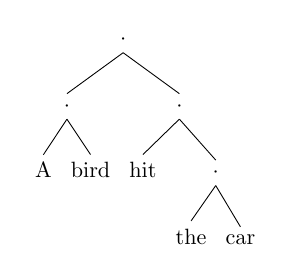
\begin{tikzpicture}[scale=.8]
    \Tree [.$\cdot$ [.$\cdot$ A bird ] [.$\cdot$ hit [.$\cdot$ the car ] ] ]
  \end{tikzpicture}
  \caption{Sentence \ref{eq:bird-brackets} as a tree. (TODO: draw this without labels.)}
  \label{fig:bird-tree}
\end{figure}
Evidence for the existence of these constituents can be provided by examples such as the following, which are called constituent tests \citep{carnie2010constituent}. Consider inserting the adverb \textit{apparently} into our example sentence, indicating the alleged status of the event described in the sentence. In principle there are six positions available for the placement of \textit{apparently} (including before, and after the sentence). However, only three of these placements are actually permissible\footnote{We use an asterisk `*' to indicate a sentence that is judged ungrammatical, as is customary in linguistics.}:
\begin{enumerate}
  \item \textit{Apparently} a bird hit the car.
  \item *An \textit{apparently} bird hit the car.
  \item A bird \textit{apparently} hit the car.
  \item *A bird hit \textit{apparently} the car.
  \item *A bird hit the \textit{apparently} car.
  \item A bird hit the car, \textit{apparently}.
\end{enumerate}
Based on the bracketing in \ref{eq:bird-brackets} we can formulate a general constraint: the adverb must not interrupt any constituent. Indeed, this explains why \textit{actually} cannot be placed anywhere inside \textit{hit the car} and not between \textit{a} and \textit{bird}. For full support, typically results from many more such test are gathered, and in general these tests can be much more controversial than in our simple example \citep{carnie2010constituent}.

\paragraph{Syntactic categories} The constituents of a sentence belong to a limited range of types that form the set of syntactic categories \citep{huddleston2002grammar}. Two types are distinguished: lexical categories (part of speech) and phrasal categories. The tree in figure \ref{fig:bird-tree} can be represented in more detail by adding syntactic categories, see figure \ref{fig:bird-tree-labeled}.
\begin{figure}[h]{\textwidth}
  \center
  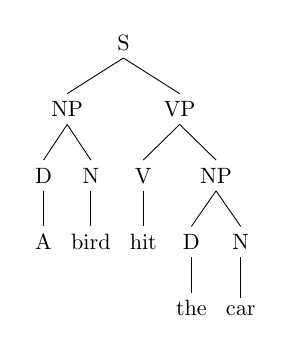
\begin{tikzpicture}[scale=.8]
    \Tree [.S [.NP [.D A ] [.N bird ]] [.VP [.V hit ] [.NP [.D the ] [.N car ] ] ] ]
  \end{tikzpicture}
  \caption{A tee specified with lexical (D, N, V) and phrasal categories (S, NP, VP).}
  \label{fig:bird-tree-labeled}
\end{figure}

\begin{figure}[b]
  \begin{subfigure}[b]{0.5\textwidth}
		\includegraphics[width=0.9\textwidth]{trees/npi-licensed.pdf}
    \label{fig:tree-npi-licensed}
    \subcaption{In licensing context.}
	\end{subfigure}
	\begin{subfigure}[b]{0.5\textwidth}
		\includegraphics[width=0.9\textwidth]{trees/npi-unlicensed.pdf}
    \label{fig:tree-npi-unlicensed}
    \subcaption{Not in licensing context.}
	\end{subfigure}
\caption{Negative Polarity. Figure taken from \cite{everaert2015structures}. (TODO: draw in qtree, but how to make the nested roofs?)}
\label{fig:trees-npi}
\end{figure}

\paragraph{Hierarchical structure} The constituents have specific roles in the larger parts they belong to \citep{huddleston2002grammar}. This structure provides constraints that are not explainable from the linear order of the words themselves. Consider the following example about the syntactic behaviour of \textit{negative polarity items} (NPIs)\footnote{A negative polarity item is, to first approximation, a word or group of words that is restricted to negative context \citep{everaert2015structures}. More generaly they are words that need to be licensed by a specific \textit{licencing context} \citep{giannakidou2011npi}.} such as \textit{anybody}:
\begin{enumerate}
  \item The book that I bought did \textit{not} appeal to \textit{anybody}.
  \item * The book that I bought appealed to \textit{anybody}.
\end{enumerate}
From this example we might formulate the hypothesis that the word \textit{not} must linearly precede the word \textit{anybody}. A counter example refutes this linear hypothesis:
\begin{enumerate}
  \item *The book I did \textit{not} buy appealed to \textit{anybody}.
\end{enumerate}
Instead, the constraints that govern this particular pattern depend on hierarchical structure: the word \textit{not} must ``structurally precede'' the word \textit{anybody} \citep{everaert2015structures}. Figure \label{ref:trees-npi} shows the constituent structure of both sentences. The explanation goes as follows (put this in my own words): \say{In sentence \ref{fig:trees-npi} (a) the hierarchical structure dominating \textit{not} also immediately dominates the hierarchical structure containing \textit{anybody}. In sentence \ref{fig:trees-npi} (b), by contrast, \textit{not} sequentially precedes \textit{anybody}, but the triangle dominating \textit{not} fails to also dominate the structure containing \textit{anybody}.}

\paragraph{Cognitive reality} Does all this exist in the human brain? These people say \textit{yes}: \citep{hale2001earley,levy2008expectation,brennan2016abstract}.

\paragraph{Controversy}
Theoretical syntax is rife with controversy, and wildly differing viewpoints exist. In fact, for each point made in our short discussion, the exact opposite point has been made as well:
\begin{itemize}
  \item Constituents are fundamental \citep{huddleston2002grammar,carnie2010constituent} \textit{versus} word-word relations are all you need \citep{tesniere1959elements,nivre2005dependency,hudson2010introduction}.
  \item Hierarchical structure is a core feature of language \citep{everaert2015structures} \textit{versus} sequential sentence structure has enough explanatory power \cite{frank2012hierarchical}. The claim is that (2) is cognitively more fundamental than (1),
  \begin{enumerate}
    \item [Sentences [ [can [be analysed] ] [as [hierarchically structured] ] ] ]
    \item [Sentences] [can be analysed] [as hierarchically structured]
  \end{enumerate}
  which is exactly contrary to the analyses above. This is more similar to the NLP task of \textit{chunking}, or shallow parsing.
  \item Studies in cognitive neuroscience and psycholinguistics show that human sentence processing is hierachical \citep{hale2001earley,levy2008expectation,brennan2016abstract} \textit{and} they show that it is not \citep{conway2008neurocognitive,christiansen2012similar,gillespie2011hierarchy, gillespie2013against} (selected from the survey in \citet{frank2012hierarchical}).
\end{itemize}
In this research I take a position of extreme pragmatism with respect to syntax: it is whatever our dataset says it is. Which means in our case, the Penn Treebank has the final word on the subject. And is language hierachical or linear? That is exactly what we inted to ivestigate from a statistical and computational viewpoint.

% \begin{figure}
%   \begin{subfigure}[b]{\textwidth}
%     \center
%     \begin{tikzpicture}[scale=.6]
% 		  \setbox\partbox=\hbox{\qroof{that I bought}.X }

\Tree [.X
        \qroof{The book \usebox{\partbox}}.X
        [.X
          \qroof{did \textit{not}}.X
          \qroof{appeal to \textit{anybody}}.X ]]

% \Tree [.X
%         [.X
%           The book \edge[roof]; { that I bought } ]
%         [.X
%           [.X \edge[roof]; {did \textit{not}} ]
%           [.X \edge[roof]; {appeal to \textit{anybody}} ] ] ]

%     \end{tikzpicture}
% 		\label{fig:tree-npi-licensed}
%   \end{subfigure}
%
%   \begin{subfigure}[b]{\textwidth}
%     \center
%     \begin{tikzpicture}[scale=.6]
% 		  \Tree [.X
        [.X
          The book \edge[roof]; { that I did \textit{not} buy } ]
        [.X
          [.X \edge[roof]; {did \textit{not}} ]
          [.X \edge[roof]; {appeal to \textit{anybody}} ] ] ]

%     \end{tikzpicture}
% 		\label{fig:tree-npi-unlicenced}
%   \end{subfigure}
%
% \caption{Negative Polarity.}
% \label{fig:trees-npi}
% \end{figure}


\section{Parsing}
\begin{itemize}
  \item Treebanks, in particular the Penn Treebank. Treebank preprocessing. CFGs, CNF, spans. Reference figure \ref{fig:trees-ptb}.
  \item The two conceptions of a tree: as a set of \textit{labeled spans} or as a set of \textit{anchored rules}.
  \item A labeled span is a triple $(\ell, i, j)$ of a syntactic label $\ell$ together the left and right endpoints $i$, $j$ that the label spans.
  \item An \textit{anchored rule} is a triple $(r, i, j)$ or four-tuple $(r, i, k, j)$, containing a CNF rule $r$ with span endpoints $i$, $j$, and a split-point $k$ of the left and right child $r$ is not a lexical rule.
  \item For the difference, consider the following two representations of the tree in figure \ref{fig:tree-cnf-spans} given in table \ref{tab:spans-rules}.
  \item Algorithms for parsing: global chart based, local transition based
  \item Dynamic programming inference versus search heuristics.
  \item Modelling types: generative, discriminative, log-linear, count-based, feature-based, neural network features.
\end{itemize}

% As images.
% \begin{figure}
% 	\centering
%   \begin{subfigure}{0.72\textwidth}
% 		\includegraphics[width=\textwidth]{trees/original.pdf}
%     \caption{Original Penn Treebank tree.}
% 		\label{fig:tree-original}
% 	\end{subfigure}
% 	\begin{subfigure}{0.62\textwidth}
% 		\includegraphics[width=\textwidth]{trees/simplified.pdf}
%     \caption{Function tags and traces removed.}
% 		\label{fig:tree-simplified}
% 	\end{subfigure}
% 	\begin{subfigure}{0.62\textwidth}
% 		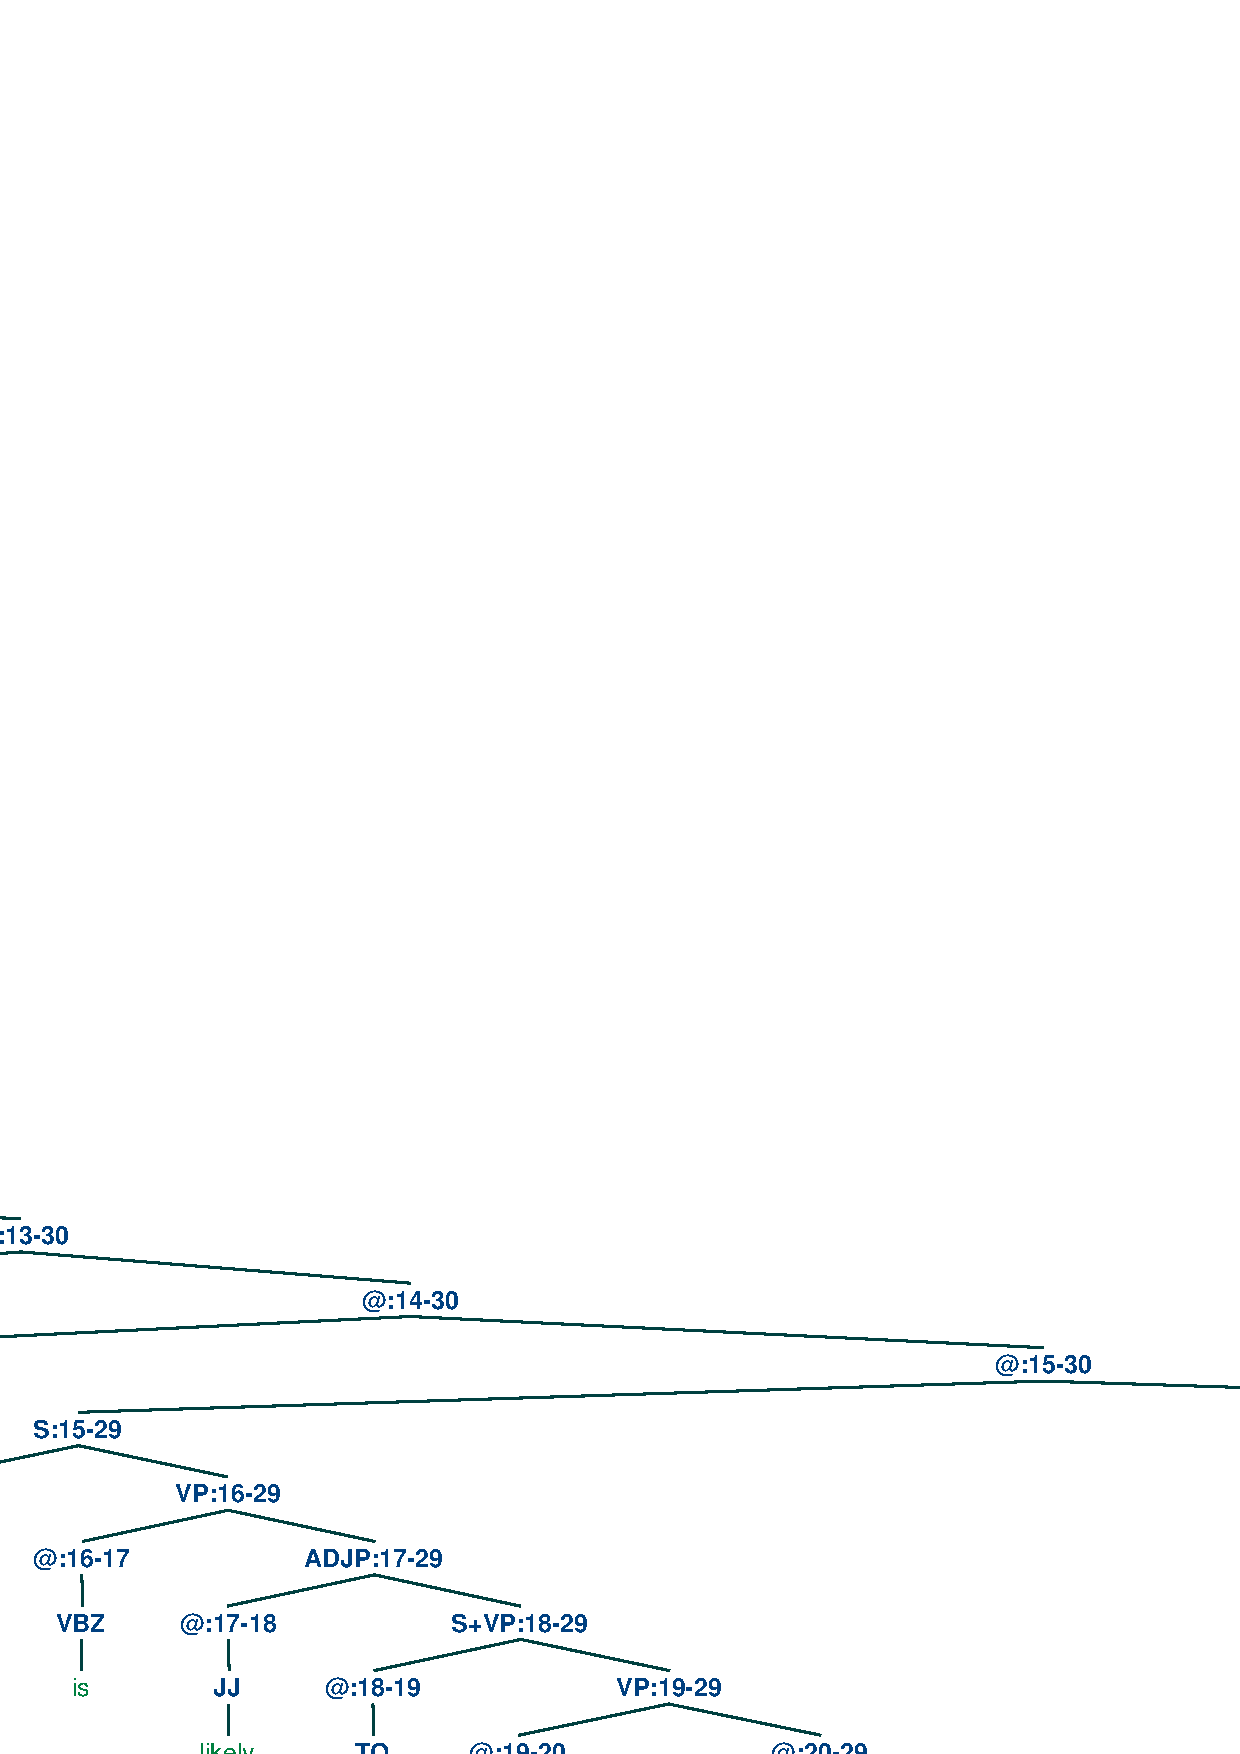
\includegraphics[width=\textwidth]{trees/binary.pdf}
%     \caption{Converted to normal form.}
% 		\label{fig:tree-cnf}
% 	\end{subfigure}
% 	\begin{subfigure}{0.9\textwidth}
% 		\includegraphics[width=\textwidth]{trees/spans.pdf}
%     \caption{In normal form with spans.}
% 		\label{fig:tree-cnf-spans}
% 	\end{subfigure}
%   \caption{Converting a treebank tree (withouth part-of-speech tags).}
%   \label{fig:trees-ptb}
% \end{figure}

\begin{figure}

  \begin{subfigure}[b]{\textwidth}
    \center
    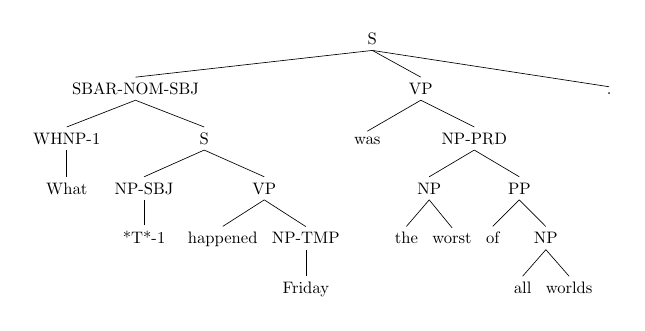
\begin{tikzpicture}[scale=.6]
      \Tree [.S
        [.SBAR-NOM-SBJ
          [.WHNP-1 What ]
          [.S [.NP-SBJ *T*-1 ] [.VP happened [.NP-TMP Friday ] ] ] ]
        [.VP
          was
          [.NP-PRD [.NP the worst ] [.PP of [.NP all worlds ] ] ] ]
        $.$ ]

    \end{tikzpicture}
    \subcaption{Original Penn Treebank tree.}
		\label{fig:tree-original}
  \end{subfigure}

  \begin{subfigure}[b]{\textwidth}
    \center
    \begin{tikzpicture}[scale=.6]
		  \input{../figures/trees/simplified.tex}
    \end{tikzpicture}
    \tiny
    \subcaption{Function tags and traces removed.}
		\label{fig:tree-simplified}
  \end{subfigure}

  \begin{subfigure}[b]{\textwidth}
    \center
    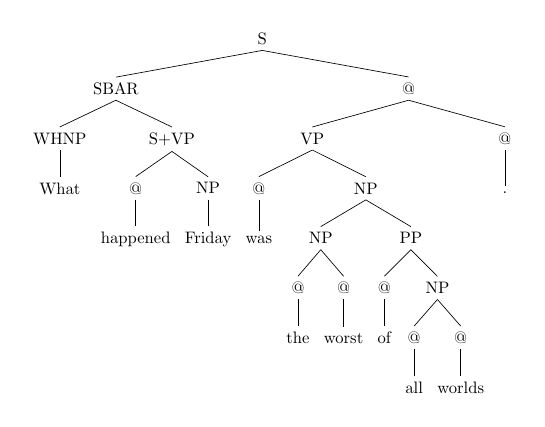
\begin{tikzpicture}[scale=.6]
		  \Tree [.S
        [.SBAR [.WHNP What ] [.S+VP [.@ happened ] [.NP Friday ] ] ]
        [.@
          [.VP
            [.@ was ]
            [.NP
              [.NP [.@ the ] [.@ worst ] ]
              [.PP [.@ of ] [.NP [.@ all ] [.@ worlds ] ] ] ] ]
          [.@ . ] ] ]

    \end{tikzpicture}
    \tiny
    \subcaption{Converted to normal form.}
		\label{fig:tree-cnf}
  \end{subfigure}

  \begin{subfigure}[b]{\textwidth}
    \center
    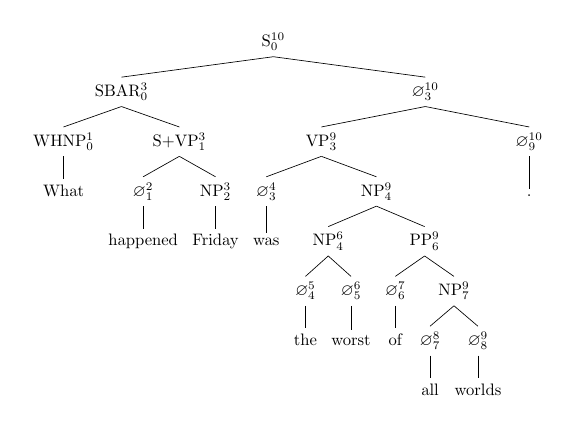
\begin{tikzpicture}[scale=.6]
		  % \Tree [.S:0-10
%         [.SBAR:0-3
%           [.WHNP:0-1 What ]
%           [.S+VP:1-3 [.$\varnothing$:1-2 happened ] [.NP:2-3 Friday ] ] ]
%         [.$\varnothing$:3-10
%           [.VP:3-9
%             [.$\varnothing$:3-4 was ]
%             [.NP:4-9
%               [.NP:4-6 [.$\varnothing$:4-5 the ] [.$\varnothing$:5-6 worst ] ]
%               [.PP:6-9
%                 [.$\varnothing$:6-7 of ]
%                 [.NP:7-9 [.$\varnothing$:7-8 all ] [.$\varnothing$:8-9 worlds ] ] ] ] ]
%           [.$\varnothing$:9-10 . ] ] ]


\Tree [.S$_0^{10}$
        [.SBAR$_0^3$
           [.WHNP$_0^1$ What ]
          [.S+VP$_1^3$ [.$\varnothing_1^2$ happened ] [.NP$_2^3$ Friday ] ] ]
        [.$\varnothing_3^{10}$
          [.VP$_3^9$
             [.$\varnothing_3^4$ was ]
            [.NP$_4^9$
               [.NP$_4^6$ [.$\varnothing_4^5$ the ] [.$\varnothing_5^6$ worst ] ]
              [.PP$_6^9$
                 [.$\varnothing_6^7$ of ]
                [.NP$_7^9$ [.$\varnothing_7^8$ all ] [.$\varnothing_8^9$ worlds ] ] ] ] ]
          [.$\varnothing_9^{10}$  . ] ] ]

    \end{tikzpicture}
    \tiny
    \subcaption{In normal form with spans.}
		\label{fig:tree-cnf-spans}
  \end{subfigure}

\caption{Converting a treebank tree (withouth part-of-speech tags).}
\label{fig:trees-ptb}
\end{figure}


\begin{table}[h]
  \center
  \small
  \bgroup  % increase vertical space
  \def\arraystretch{1.5}  % increase vertical space
  \begin{tabular}{l|l}
    Labeled spans & Anchored rules \\
    \hline
    (S, 0, 10)     & (S $\to$ SBAR $\varnothing$, 0, 3, 10)  \\
    (SBAR, 0, 3)   & (SBAR $\to$ WHNP S+VP, 0, 1, 3)  \\
    (VP, 1, 3)     & (S+VP $\to$ $\varnothing$ NP, 1, 2, 3)  \\
    $\qquad\vdots$ & $\qquad\vdots$  \\
    (NP, 7, 9)     & (NP $\to$ $\varnothing$ $\varnothing$, 7, 8, 9)  \\
  \end{tabular}
  \caption{Two conceptions of the tree in \ref{fig:tree-cnf-spans}.}
  \label{tab:spans-rules}
  \egroup  % increase vertical space
\end{table}


\section{Language models}
\begin{itemize}
  \item Briefly mention some typical approaches for langugage modelling: count based n-gram with smoothing \citep{chen1999empirical,kneser1995improved}, neural n-gram \citep{bengio2003neural} and recurrent neural network \citep{mikolov2010recurrent}. Also mention some (early) syntactic approaches: count-based \citep{chelba2000structured,pauls2012treelets}, neural \citep{emami2005neural}, and top-down parsing related \citep{roark2001probabilistic}.
  \item Explain the metric perplexity.
  \item Briefly mentions some typical datasets and some benchmarks (dataset, perplexity, number of parameters, training time).
  \item Mention some downsides of the perplexity metric: conflating different sources of succes in next-word prediction (simple collocations, semantics, syntax).
  \item Note that there exists some alternatives to perplexity: adversarial evaluation \citep{smith2012adversarial}, subject-verb agreement \citep{linzen2016syntax} and grammatical acceptability judgments \citep{linzen2018targeted}.
\end{itemize}


\section{Neural networks}
Introduce all the neural networks.
\begin{itemize}
  \item We consider the neural networks as abstractions denoting certain parametrized functions \ff, \rnn, \lstm, etc.
  \item Let $\x$ and $\y$ be vectors in respectively $\reals^{n}$ and $\reals^{m}$.

  A \textit{feedforward neural network} is a parametrized function $\ff$ from $\reals^{n}$ to $\reals^{m}$ such that
  \begin{align*}
    \ff( \x ) &= \y.
  \end{align*}

  A \textit{recurrent neural network} is a parametrized function \rnn that takes a sequence of vectors $(\x_i)_{i=1}^n = ( \x_1, \x_2, \dots, \x_n )$ in $\reals^{n}$ and produces a sequence of output vectors in $( \y_1, \y_2, \dots,\y_n )$ in $\reals^{m}$:
  \begin{align*}
    \rnn( (\x_i)_{i=1}^n ) &= ( \y_1, \y_2, \dots, \y_n ).
  \end{align*}
  Internally, the \rnn recursively applies a function $f: \reals^{n} \times \reals^{m} \to \reals^{m}$ that is defined by the recursion
  \begin{align*}
    \y_{t} &= f(\x_t, \y_{t-1})  \\
      &= f(\x_t, f(\x_{t-1}, \y_{t-2}))  \\
      &\;\vdots \\
      &= f(\x_t, f(\x_{t-1}, f(\dots f(\x_{1}, \y_{0})))),
  \end{align*}
  which is how the vectors $\y_i$ are computed. That is, $f$ takes the input $\x$ of the current timestep $t$ and the output $\y$ of the previous timestep $t-1$ and returns a new ouput for timestep $t$. The initial vector $\y_{0}$ does not depend on the input, and can be fixed or part of the function's set of parameters.

  An \rnn can be applied to the input sequence in reverse, that is, in the \textit{backward} direction:
  \begin{align*}
    \rnn_B( (\x_i)_{i=1}^n )
      &= \rev( \rnn( \rev( (\x_i)_{i=1}^n ) ) ) \\
      &= \rev( \rnn( \x_n, \x_{n-1}, \dots, \x_1 ) \\
      &= \rev( \y_n, \y_{n-1}, \dots, \y_1 ) \\
      &= (\y_1,\y_2, \dots, \y_n ), \\
  \end{align*}
  where we defined a
  \begin{equation}
    \rev( (\x_i)_{i=1}^n ) \defeq ( \x_n, \x_{n-1}, \dots, \x_1 ),
  \end{equation}

  For consistency we will refer to the \rnn in the regular, \textit{forward}, direction as $\rnn_F$. To stress the difference between the different outputs obtained from the two directions, we will denote the output vectors obtained in the regular, forward, direction with $\fw_i$ and the vectors obtained in the backward direction with $\bw_i$:
  \begin{align*}
    \rnn_F( (\x_i)_{i=1}^n ) &= ( \fw_1, \fw_2, \dots, \fw_n ) \\
    \rnn_B( (\x_i)_{i=1}^n ) &= ( \bw_1, \bw_2, \dots, \bw_n )
  \end{align*}
  The two functions above can used to construct a \textit{bidirectional} \rnn by combining the output of each as
  \begin{equation}
    \birnn( (\x_i)_{i=1}^n ) = ( \fw_1 \concat \bw_1, \fw_2 \concat \bw_2, \dots, \fw_n \concat \bw_n ),
  \end{equation}
  where we use $\concat$ to denote vector concatenation, \ie $\x \concat \y$ is a vector in $\reals^{n+m}$.

  An \lstm is a particular way to construct the \rnn internal function $f$, and similarly has a bidirectional equivalent denoted \bilstm.
  \item The function \ff is defined as follows:
  \item The function \lstm is defined as follows
  \item (Minibatch) SGD optimization.
\end{itemize}



\chapter{Recurrent Neural Network Grammars}
\label{03-rnng}
% \bibliography{../src/bibliography}

\section{Model}
I describe the model.
\begin{itemize}
  \item Specify the transition-system.
  \item The probabilistic model is given by
  \begin{equation}
    p(\mathbf{x}, \mathbf{y}) = \prod_{t=1}^A p(a_t | \mathbf{a}_{<t}) p(w_{W(t)} | \mathbf{a}_{<t} )^{ \mathbb{I}[a = \textsc{gen}] } p(n_{N(t)} | \mathbf{a}_{<t} )^{ \mathbb{I}[a = \textsc{open}] },
  \end{equation}
  where $\dots$
\end{itemize}

\subsection{Features}
The features from which the transition probabilities are predicted are computed from the entire transition history (no markov assumption) and in a syntax dependent way.
\begin{itemize}
  \item The StackLSTM computes incremental features for the sequences on the three datastructures of the transition-system, with unbounded history.
  \item A composition function computes representations of closed constituents.
  \item There are two options for the composition function: simple BiRNN and attention-based. The attention-based composition performed best in earlier research, so we focus on this composition.
  \item There is evidence that the stack- is all that is needed. We focus on the models that compute representations of all the datastructures.
\end{itemize}

\section{Syntax and cognition}
Here I describe the research into syntax and cognition using the RNNG.

\paragraph{Cognition} RNNGs can tell us something about our brains.
\begin{itemize}
  \item Psycholinguistic research that indicates that top-down parsing is a cognitively plausible parsing strategy \citep{Brennan+2016}.
  \item RNNGs are good statistical predictors in psycholinguistic research \citep{Hale+2018:beam}. More precise: the sequential word-probabilities that are derived from a generative RNNG with word-synchronous beam-search \citep{Stern+2017:beam} provide complexity metrics that predict human reading difficulty well.
\end{itemize}

\paragraph{Syntax} What do RNNGs learn about syntax?
\begin{itemize}
  \item RNNGs learn a number of syntactic phenomena as a side product of the main objective. The attention mechanism in the composition function learns a type of `soft' head-rules, and when trained on trees without syntactic labels the RNNG still learns representations for constituents that cluster according to their withheld gold label \citep{Kuncoro+2017:RNNG-syntax}.
  \item RNNGs are better at a long-distance verb-argument agreement task than LSTMS \cite{Linzen+2016:LSTM-syntax,Kuncoro+2018:RNNG-deps}.
\end{itemize}

\section{Experiments}
We perform three types of experiments with the RNNG:
\begin{itemize}
  \item We reproduce the parsing f-scores and perplexities from \citep{Dyer+2016:RNNG}, and some more.
  \item We evauluate `how good the model is' as a sampler.
\end{itemize}

\paragraph{Supervised model} We investigate the following.
\begin{itemize}
  \item We train with standard hyperparameter settings and optimizer, and replicate the original results. We will get a little lower with the discriminative model because we do not use tags.
  \item We evaluate F-score with 100 samples (as many proposal trees as possible).
  \item We evaluate perplexity with varying number of samples: 1 (argmax), 10, 20, 50, 100 (default). The peplexity evaluation with the argmax prediction gives an impression of the uncertaty in the model \citep{Buys+2018}.
\end{itemize}

\paragraph{Sampler} We investigate the following:
\begin{itemize}
  \item We asses the conditional entropy of the model. This is most quantitative. Recall that conditional entropy is defined as
  \begin{equation}
    \text{H}(Y|X) = \sum_{x \in \mathcal{X}} p_X(x)\text{H}(Y|X = x),
  \end{equation}
  where
  \begin{equation}
    \text{H}(Y|X = x) = - \sum_{y \in \mathcal{Y}} p_{Y|X}(y|x) \log p_{Y|X}(y|x).
  \end{equation}
  We estimate the quantity $\text{H}(Y|X = x)$ with the model samples. We estimate the quantity $\text{H}(Y|X)$ by a sum over the development dataset. For the probabilities $p_X(x)$ we use the marginalized probabilities of the joint RNNG (with samples from the discrminative parser $p_{Y|X}$).
  \item We asses for some cherry picked sentences. This is more qualitative. These sentences should be difficult or ambiguous. Or they can be ungramatical when taken from the syneval dataset. We can evaluate their entropy, and the diversity of samples, for example to see if there are clear modes. We can make violinplots of the probabilities of the samples. We can compute the f-scores of the samples compared with the argmax tree.
\end{itemize}


\section{Related work}
\begin{itemize}
  \item Generative dependency parsing and language modelling \citep{Buys+2015:bayes-gen-dep,Buys+2015:neural-gen-dep,Buys+2018}
  \item Top-down parsing and language modelling \citep{Roark2001}.
  \item Brains research with top-down parsing \citep{Hale+2018:beam,Brennan+2016}.
\end{itemize}



\chapter{Conditional Random Field parser}
\label{04-crf}
% \bibliography{../src/bibliography}

This chapter introduces a neural Conditional Random Field (CRF) parser that can be used as an alternative proposal distribution for the approximate marginalization of the RNNG. The model is a span-factored CRF that independently predicts scores for labeled spans over the sentence using neural networks. The scores then interact in a chart-based dynamic program, giving a compact description of the probability distribution over parses. This approach combines the efficient exact inference of chart-based parsing, the rich nonlinear features of neural networks, and the global training of a CRF. The chart-based approach allows efficient exact inference alowing for exact decoding and global sampling while the neural features can be complex and can condition on the entire sentence. The CRF training objective [...something about receiving information about all substructures...]. The parser is an adaptation of the chart-based parser introduced in \citet{stern2017minimal} to global CRF training. \citet{stern2017minimal} train the model with a margin-based objective, but our interest primary in this model is as a proposal distribution, which requires probabilistical training.

In this chapter:
\begin{itemize}
  \item I present the parser and describe how it is an adaptation of earlier log-linear and neural crf parsing \citep{finkel2008crf,klein2015crf} and the maximum margin trained parser of \citet{stern2017minimal}.
  \item I show how the several inference problems of interest can be solved exactly: prediction, entropy, sampling.
  \item We train the parser in a supervised fashion and show it's adequacy as a parser.
  \item We invesitage the kind of samples that are obtained from this parser, and evaluate how they affect the approximate inference in the RNNG.
\end{itemize}


\section{Model}
The model is a CRF factored over the labeled spans that form a tree. Let $x$ be a sentence, and $y$ a tree from $\yieldx$. We define a function $\Psi$ that assings nonnegative scores $\Psi(\x, \y)$ and let the probability of a tree be its globally normalized score
\begin{align}
  \label{eq:crf-model}
  p(\y \mid \x) &= \frac{\Psi(\x, \y)}{Z(\x)},
\end{align}
where
\begin{align*}
  Z(\x) = \sum_{ \y \in \yieldx } \Psi(\x, \y).
\end{align*}
is the normalizer, or partition function, that sums over the exponential number of trees availlable for $\x$.

To allow efficient computation of the normalizer, we let the scoring function $\Psi$ factorize over the parts of $\y$. We consider a tree as a set of labeled spans $\y_a = (A, i, j)$, thus $\y = \{ \y_a \}_{a=1}^A$, where $(A, i, j)$ indicates that $\y$ contains a label $A$ spanning the words $\langle x_{i+1}, \dots, \x_j \rangle$. The value $\Psi(\x, \y)$ is then defined as the product of the nonnegative potentials $\psi(\x, \y_a)$ of the parts of $\y$
\begin{align}
  \Psi(\x, \y) = \prod_{a=1}^A \psi(\x, \y_a).
\end{align}
The function $\psi$ thus scores each labeled span $\y_a$ seperately, but conditional on the entire sentence.

The above model is your typical constituency parsing CRF \citep{finkel2008crf,klein2015crf}, but the factorization over labeled spans, however, was first introduced by \citet{stern2017minimal}. By factorizing a tree over labeled spans we make an even stronger assumption than that typically made by factorizating over anchored context-free rules\footnote{\cf table \ref{tab:spans-rules} for the different conceptions.}, such as is done in \citet{finkel2008crf,klein2015crf}. By factorizing over labeled spans, the potential function has no access to information about the direct substructure under the node, such as the child nodes and their split point. The function can thus rely less on the local tree structure and must thus rely more on the surface features of input sentence. This factorization will, however, greatly reduce the size of the state-space of the dynamic programs, speeding up training and inference, and the burden of the feature function will be carried by a rich neural network parametrization. Together, this will make the parser fast and very effective.

\section{Parametrization}
The scoring function $\psi$ is implemented with neural networks following \citet{stern2017minimal}. The local potentials can only make minimal use of structural information, as we argued above, but they can depend on the entire sentence. This suggest the use of RNN encodings. We let the representation of a span $(i, j)$ be the concatenation of the difference between forward and backward vectors
\begin{align}
  \label{eq:span-feature}
  \vecs_{ij} = [\fw_j - \fw_i; \bw_i - \bw_j],
\end{align}
illustrated in figure \ref{fig:span-feature}. The score for a label $A$ then, is computed from this vector using a feedforward network:
\begin{align}
  \label{eq:potential-function}
  \log \psi(\x, \y_a) = [ \ff( \vecs_{ij} ) ]_{A}.
\end{align}
This architecture is rightly called minimal, but it works surprisingly well: \citet{stern2017minimal} experiment with more elaborate functions based on concatenation of vectors (a strict superset of the minus approach) and biaffine scoring (inspired by \citep{dozat2016deep}), but these function improve marginally, if they do at all.

\begin{figure}
  \includegraphics[width=\textwidth]{span-encoding.pdf}
  \caption{Representation for the span $(1, 4)$ computed from $\rnn$ encodings. Taken without permission from \citet{stern2018analyis}.}
  \label{fig:span-feature}
\end{figure}

\section{Inference}
Because the model is span-factored it allows efficient inference. In this section we describe efficient solutions to four related problems:
\begin{itemize}
  \item Compute the normalizer $Z(\x) = \sum_{ \y \in \yieldx } \prod_{ a=1 }^{ A } \psi( \x, \y_a )$.
  \item Find the best parse $\hat{ \y } = \arg \max_{\y } p(\y  \mid \x)$
  \item Obtain a sample $y \sim p(\cdot \mid \x)$.
  \item Compute the entropy $H(P(Y \mid X = x))$ over parses for $\x$.
\end{itemize}
These problems are solved by variants of the inside and outside algorithms. We first describe how the quantities computed by these algorithms will be used to solve these problems, and then how these are computed.

\subsection{Quantities}
  For each labeled span $(A, i, j)$, we define the inside value $\alpha(A, i, j)$ as the sum of potentials of all trees that are rooted in node $A$ with leaves $x_{i+1} \dots x_j$. We define the outside value $\beta(A, i, j)$ as the sum over potentials of all trees with leaves $x_1 \dots x_i A x_{j+1} \dots x_n$, where the nonterminal $A$ is treated as a leaf that is not expanded. These values sum over complementary sets that together make up all parses of $\x$.

  % We then define the quantity $\mu(A, i, j)$ as the sum of all parses of $\x$ that contain nonterminal $\y_a = (A, i, j)$:
  % \begin{align*}
  %   \mu(i, j, \ell)
  %     &\defeq \sum_{ \substack{ \y \in \yieldx \\ \y_a \in \y } } \psi(\x, \y_a),
  % \end{align*}
  % and note that under this these definition we have the result
  % \begin{align}
  %   \mu(A, i, j) &= \alpha(A, i, j) \beta(A, i, j).
  % \end{align}
  % Given these quantities, we can directly solve three problems described above.

  \paragraph{Normalizer}
    The normalizer is the inside value at the root node
    \begin{align}
      Z(\x) = \alpha(\text{S}^{\dagger}, 0, n),
    \end{align}
    which follows from the definition of the inside algorithm: $\alpha(\text{S}^{\dagger}, 0, n)$ is the sum of potentials of all trees rooted in $\text{S}^{\dagger}$ that span words $x_1 \dots x_n$.

  \paragraph{Marginals}
    The posterior marginal is the probability that a labeled span $\y_a$ occurs in a tree $\y$ for the sentence $\x$ as governed by the distribution $p$. We can write this as
    \begin{align}
      P(Y_a = \y_a \mid X = \x)
        &= \expect[ \indicator_{ \{ \y_a \in Y \} } ]  \\
        &= \sum_{ \y \in \yieldx } p(\y \mid \x) \indicator_{ \{ \y_a \in Y \} }
    \end{align}
    and abbreviate this probability mnemonically as $\mu(\y_a \mid \x)$. A clasical result is that
    \begin{align}
      \mu(\y_a \mid \x) = \frac{\alpha(A, i, j) \cdot \beta(A, i, j)}{Z(\x)},
    \end{align}
    which can be seen by noting that $\alpha(A, i, j) \cdot \beta(A, i, j)$ is the sum over all trees that contain the node $\y_a$, and $Z(\x)$ the sum over all trees in general.

  \paragraph{Entropy}
    The entropy of the distribution over parses can be computed efficiently using the node marginals. We derive
    \begin{align*}
      H(P_{Y \vert X = x})
        &= - \sum_{ \y \in \yieldx } p(\y \mid \x) \log p(\y \mid \x)  \\
        &= \log Z(\x) - \sum_{ \y \in \yieldx } p(\y \mid \x) \sum_{\y_a \in \y} \log \psi(\x, \y_a)  \\
        &= \log Z(\x) - \sum_{ \y \in \yieldx } p(\y \mid \x) \sum_{ a \in \mathcal{A}(x) } \indicator_{ \{ \y_a \in Y \} } \log \psi(\x, a)  \\
        &= \log Z(\x) - \sum_{ a \in \mathcal{A}(x) } \log \psi(\x, a)  \sum_{ \y \in \yieldx } \indicator_{ \{ \y_a \in Y \} } p(\y \mid \x)  \\
        &= \log Z(\x) - \sum_{ a \in \mathcal{A}(x) } \log \psi(\x, a)  \mu(a \mid \x)  \\
        &=  \log Z(\x) - \expect_{ \mu } \Big[ \log \psi(\x, a) \Big]  \\
    \end{align*}

  \paragraph{Parse}
    The best parse can be obtained with the Viterbi algoritm, which is an instance of the inside algorithm. The viterbi algorithm replaces the sum operator of the inside algorithmm with $\max$: at each node this selects the best substructure instead of summing over all of them.

\subsection{Inside recursion}
  The inside algorithm computes the quantities $\alpha(A,i,j)$ for all labels $A \in \Lambda$ and all spans $0 \leq i < j \leq n$. From the hypergraph perspecive this is the total weight under the node $v = (A, i, j)$---the sum of the weights of all directed paths incoming at $v$. This sum can be computed using the \textit{inside recursion} \citep{goodman1999semiring}.

  At the nodes that span one word, the inside value is just the weight of the unary edge
  \begin{align}
      \label{eq:inside-base}
      \alpha(A, i, i+1) = \psi(A, i, i+1)
  \end{align}
  for $A \in \Lambda$, for all $0 \leq i < n$.

  To compute $\alpha(A, i, j)$ in the general case we need to sum over all possible binary expansions $(A \to B C, i, k, j)$ for $A, B \in \Lambda$ and $i \leq k \leq j$. This corresponds to the following recursive expression that uses the inside values of the subparts:
  \begin{align*}
    \label{eq:inside}
    \alpha(A, i, j)
      &= \bigoplus_{B \in \Lambda} \bigoplus_{C \in \Lambda} \bigoplus_{k=i+1}^{j-1} \psi(A, i, j) \otimes \alpha(B,i,k) \otimes \alpha(C,k,j) \\
      &= \psi(A, i, j) \otimes \bigoplus_{k=i+1}^{j-1} \bigoplus_{B \in \Lambda} \alpha(B,i,k) \otimes \bigoplus_{C \in \Lambda} \alpha(C,k,j) \\
      &= \psi(A, i, j) \otimes \bigoplus_{k=i+1}^{j-1} S(i,k) \otimes S(k,j)
  \end{align*}
  where we've introduced the notational abbreviation
  \begin{align*}
      S(i,j) &= \bigoplus_{A \in \Lambda} \alpha(A,i,j).
  \end{align*}
  Looking at \ref{eq:inside} we can see the marginalized values $S(i, j)$ are all that are needed for the recursion. This suggest simplifying the recursion even further as
  \begin{align*}
    \label{eq:inside-simplified}
    S(i, j)
      &= \bigoplus_{A \in \Lambda} \alpha(A,i,j) \\
      % &=  \bigoplus_{A \in \Lambda} \psi(A, i, j) \otimes \bigoplus_{k=i+1}^{j-1} S(i,k) \otimes S(k,j) \\
      &= \Bigg[ \bigoplus_{A \in \Lambda} \psi(A, i, j) \Bigg] \otimes \Bigg[\bigoplus_{k=i+1}^{j-1} S(i,k) \otimes  S(k,j) \Bigg],
  \end{align*}
  where we put explicit brackets to emphasize that independence of the subproblems of labeling and splitting.

  This recursion can be solved by computing the inside value of the nodes $(i, j, A)$ in topological order, so that the values of the subparts are availlable to compute the inside values higher up.

\subsection{Outside recursion}
  The outside algorithm computes the quantities $\beta(A,i,j)$ for all labels $A \in \Lambda$ and all spans $0 \leq i < j \leq n$. For the labels spanning the entire sentence, the outside value is defined as
  \begin{align*}
    \beta(A, 0, n) =
    \begin{cases}
      \hat{1}, & \text{ if } A = \text{S}^{\dagger}  \\
      \hat{0}, & \text{otherwise}.
    \end{cases}
  \end{align*}
  To compute $\beta(A, i, j)$ in the general case we need to sum over all possible upward binary expansions that $A$ can be a part of, recursively making use of the outside values already computed. This means we sum over expansions $(B \to C \; A, k, i, j)$ for all labels $B$ and $C$ and left endpoints $1 \leq k < i$, and sum over expansions $(B \to A \; C, i, j, k)$ for all labels $B$ and $C$ and right endpoints $j < k \leq n$. This corresponds to the following recursive expression that uses the outside values of the superparts:
  \begin{align*}
    \beta(A, i, j)
      &= \bigoplus_{B \in \Lambda} \bigoplus_{C \in \Lambda} \bigoplus_{k=1}^{i-1} \psi(B, k, j) \otimes \alpha(C, k, i-1) \otimes \beta(B, k, j) \\
        &\qquad \oplus \bigoplus_{B \in \Lambda} \bigoplus_{C \in \Lambda} \bigoplus_{k=j+1}^{n} \psi(B, i, k) \otimes \beta(B, i, k) \otimes \alpha(C, j+1, k) \\
      &=  \bigoplus_{k=1}^{i-1}  \Bigg[ \bigoplus_{B \in \Lambda} \psi(B, k, j)  \otimes \beta(B, k, j) \Bigg] \otimes \Bigg[ \bigoplus_{C \in \Lambda} \alpha(C, k, i-1) \Bigg] \\
        &\qquad \oplus \bigoplus_{k=j+1}^{n}  \Bigg[ \bigoplus_{B \in \Lambda}  \psi(B, i, k) \otimes \beta(B, i, k) \Bigg] \otimes  \Bigg[  \bigoplus_{C \in \Lambda} \alpha(C, j+1, k) \Bigg] \\
      &=  \bigoplus_{k=1}^{i-1}  S'(k, j) \otimes S(k, i-1) \oplus \bigoplus_{k=j+1}^{n} S'(i, k) \otimes  S(j+1, k) \\
  \end{align*}
  where
  \begin{align*}
      S(i, j) &= \bigoplus_{A \in \Lambda} \alpha(A, i, j) \\
      S'(i, j) &= \bigoplus_{A \in \Lambda} \psi(A, i, j) \beta(A, i, j)
  \end{align*}

\subsection{Viterbi recursion}
  To ontain the viterbi tree and its probability we use the Viterbi semirings. The score of the best tree is computed by replacing the sum with the $\max$ in equation
  \begin{align}
  \label{eq:viterbi-score}
    \nu(i,j)
      &= \max_{A} [ \psi(A, i, j) ] \cdot \max_{k} [\nu(i,k) \cdot \nu(k,j)].
  \end{align}
  Since these maximization over label and over split point is independent, we can find them seprately
  \begin{align}
  \label{eq:viterbi-tree}
    \hat{A} &= \argmax_{ A  } \psi(A, i, j)  \\
    \hat{k} &= \argmax_{ k } \nu(i, k) \cdot \nu(k, j)
  \end{align}
  The best tree is then found by following back the best splits an labels from the root.

% \subparagraph{Numerical concerns}
%   The above recursion computes the result of exponentially many additions and multiplications. This will soon run into the problem of numerical underflow and overflow. Instead, we compute these quantities in the logarithmic domain, defining the $\oplus$ as
%   \begin{align*}
%     a \osum b = \log(e^{a} + e^{b}),
%   \end{align*}
%   and $\otimes$ as
%   \begin{align*}
%     a \otimes b = a + b.
%   \end{align*}
%   The definition of $\oplus$ is made numerically stable by writing
%   \begin{align*}
%     \log(e^{a} + e^{b} = a + \log(1 + e^{b-a}) = b + \log(1 + e^{a-b})
%   \end{align*}
%   and choosing expression with the smaller exponent.

\section{Experiments}
  We perform three types of experiments with the CRF parser:
  \begin{itemize}
    \item We show that the model is a good supervised parser. We train the model supervised on the PTB and show the f-score on the PTB test set.
    \item We evaluate the joint RNNG with samples from the CRF parser. We compare the perplexity and fscore with RNNG case.
    \item We evauluate `how good the model is' as a sampler.
  \end{itemize}

\subsection{Supervised model} We investigate the following.
  \begin{itemize}
    \item We have some optimization and hyperparameter choices here. The original paper uses Adam with 0.001 and a LSTM of dimension 250, which gives the model around 2.5 million parameters. For the discriminative RRNG we use SGD with 0.1, and hidden sizes of 128 gives the model around 800,000 parameters.
    \item I suggest two experiments: (1) use the default setting from \citep{stern2017minimal} and (2) use the settings for the RNNG with a hidden size to match the 800,000 parameters.
  \end{itemize}

\subsection{Proposal model} We investigate the following:
  \begin{itemize}
    \item We evaluate validation F-score and perplexity.
    \item We evaluate F-score with 100 samples (as many proposal trees as possible).
    \item We evaluate perplexity with varying number of samples: 1 (argmax), 10, 20, 50, 100 (default). The peplexity evaluation with the argmax prediction gives an impression of the uncertaty in the model \citep{buys2018exact}.
    \item  We perform learning rate decay and model selection based on a development score computed with the samples from the discriminative RNNG. Undecided: should we train a separate joint RNNG with CRF samples?
  \end{itemize}

\subsection{Sampler} We investigate the following:
  \begin{itemize}
    \item We asses the conditional entropy of the model. This is most quantitative. Recall that conditional entropy is defined as
    \begin{equation}
      \text{H}(Y|X) = \sum_{x \in \mathcal{X}} p_X(x)\text{H}(Y|X = x),
    \end{equation}
    where
    \begin{equation}
      \text{H}(Y|X = x) = - \sum_{y \in \mathcal{Y}} p_{Y|X}(y|x) \log p_{Y|X}(y|x).
    \end{equation}
    The quantity $\text{H}(Y|X = x)$ can computed exactly with the CRF parser. We estimate the quantity $\text{H}(Y|X)$ by a sum over the development dataset. For the probabilities $p_X(x)$ we use the marginalized probabilities of the joint RNNG (with samples from the CRF parser $p_{Y|X}$).
    \item We asses for some cherry picked sentences. This is more qualitative. These sentences should be difficult or ambiguous. Or they can be ungramatical when taken from the syneval dataset. We can evaluate their entropy, and the diversity of samples, for example to see if there are clear modes. We can make violinplots of the probabilities of the samples. We can compute the f-scores of the samples compared with the argmax tree.
  \end{itemize}

\section{Related work}
Here I describe related work, and in particular earlier approaches to (neural) CRF-parsing.
\begin{enumerate}
  \item Of course \citep{stern2017minimal}
  \item CRFs \citep{sutton2012crf}
  \item CRF parsing with linear and nonlinear features \citep{finkel2008crf,klein2015crf}
  \item Attempts to simplify the grammar and thus the state-space of the dynamic program \citep{hall2014less}.
  \item Recent extension of \citet{stern2017minimal}, with same model but different features \citep{kitaev2018attentive}.
\end{enumerate}

\subsection{Motivation}
The model regards a constituency tree as a collection of \textit{labeled spans} over a sentence. Earlier CRF models for constituency parsing, both log-linear and neural, factorize trees over \textit{anchored rules} \citep{finkel2008crf,klein2015crf}. This puts most of the expressiveness of the model in the state space of the dynamic program, modelling interactions between subparts of the trees through their interaction in the rules, instead of at the feature level. The model in \citet{stern2017minimal} removes part of this structure, and puts more expressiveness in the input space by using rich neural feature representations conditioning on the entire sentence. The discrete interaction between the local scores remains only at level of labeled spans. This dramatically improves the speed of this model, which will become evident in the next section.

Chart based parsing has moved from grammar to features: the work of \citet{hall2014less} shows how the log-linear CRF model of \cite{finkel2008crf} can work with bare unnanotated grammars, when relying more on the surface features of the sentence, and \citet{klein2015crf} show how these surface features can be replaced with dense neural features. The work of \citep{stern2017minimal} moves one step further: the grammar is dispensed with altogether, making the model span-factored, and the scoring function is given the full power of neural networks.

Contrast this with generative parsing based on treebank grammars, where features are not available because the models are not conditional. Instead, these models rely entirely on detailed rule information: basic treebank grammars do not parse well because the rules provide too little context, and good results can only be obtained by enriching grammars. The independence assumptions in the grammar are thus typically weakened, not strengtehened. Such approaches lexicalize rules \citep{collins2003head}, annotate the rule with parent and sibling labels \citep{klein2003accurate}, or automatically learn refinements of nonterminal categories \citep{petrov2006learning}.

The closest predecessor to our model is the neural CRF parser of \citet{klein2015crf}, which predicts local potential for anchored rules using a feedfoward network. This differs from our approach in two ways. Their method requires a grammar, extracted from a treebank beforehand, whereas our approach implictly assumes all rules are possible rules in the grammar. Secondly, their scoring function conditions only on the parts of the sentence directly under the rule, dictated by the use of a feedforward network, whereas our scoring function computes a score bassed on representations computed from the entire sequence.

Earlier work on CRF parsing consider a tree as a collection of anchored rule productions productions \cite{finkel2008crf,klein2015crf}, and hence define the score of a tree as the product over clique potentials on anchored rules:
\begin{align}
  \log\psi(A \to B \;C, i, k, j) = \log\psi(A, i, j)\\
\end{align}
discarding the rest of the span information. The function is then defined as
\begin{align}
  \label{eq:span-score}
  \log\psi(A, i, j) &\defeq s(i, j, A),
\end{align}
Note that the potential function as defined in \ref{eq:rule-score} disregards most of the information in a binary rule. In particular we see that $B$, $C$ and $k$, the labels and split-point of the children, are discarded.


% \subsection{Inside recursion}
% In this derivation we will use $\y_a = (i, j, \ell)$ interchangeably.
%
% \begin{align*}
% \label{eq:inside}
%   \alpha(A,i,j) &= \sum_{B \in N} \sum_{C \in N} \sum_{k=i+1}^{j-1} \tilde{s}(i, j, A) \cdot \alpha(B,i,k) \cdot \alpha(C,k,j) \\
%     &= \tilde{s}(i, j, A) \cdot \sum_{k=i+1}^{j-1} \sum_{B \in N} \alpha(B,i,k) \cdot \sum_{C \in N} \alpha(C,k,j) \\
%     &= \tilde{s}(i, j, A) \cdot \sum_{k=i+1}^{j-1} S(i,k) \cdot S(k,j)
% \end{align*}
%
% where we've introduced a number of notational abbreviations
% \begin{align*}
%   \tilde{s}(i, j, A)
%     &= \exp( s(i, j, A) ) \\
%     S(i,j) &= \sum_{A \in N} \alpha(A,i,j)
% \end{align*}
%
% From equation \ref{eq:inside} we can deduce that we in fact do even need to store the values $\alpha(i, j, A)$ but that it suffices to only store the marginalized values $S(i, j)$. In this case, the recursion simplifies even further:
% \begin{align*}
%     S(i, j) &= \sum_{A \in N} \alpha(A,i,j) \\
%         &=  \sum_{A \in N} \tilde{s}(i, j, A) \cdot \sum_{k=i+1}^{j-1} S(i,k) \cdot S(k,j) \\
%         &= \Bigg[ \sum_{A \in N} \tilde{s}(i, j, A) \Bigg] \cdot \Bigg[\sum_{k=i+1}^{j-1} S(i,k) \cdot  S(k,j) \Bigg]
% \end{align*}
% where we put explicit brackets to emphasize that independence of the subproblems of labeling and splitting.
%
% \subsection{Inside recursion}
% In this derivation we follow Michael Collins notes on the Inside-Outside Algorithm.\footnote{\url{http://www.cs.columbia.edu/~mcollins/io.pdf}} We have the following general result for the inside value $\alpha$. For all $A \in N$, for all $0 \leq i < n$
% \begin{align}
%     \label{eq:collins-inside-base}
%     \alpha(A,i,i+1) = \psi(A, i, i+1)
% \end{align}
% and for all $(i, j)$ such that $1 \leq i < j \leq n$:
% \begin{align}
%     \label{eq:collins-inside-general}
%     \alpha(A,i,j) = \sum_{A \to B C} \sum_{k=i+1}^{j-1} \psi(A \to B \;C, i, k, j) \cdot \alpha(B,i,k) \cdot \alpha(C,k,j)
% \end{align}
% Note that we are considering a CFG in which the rule set is complete, i.e.
% \begin{align}
%   \langle A \to B \;C \rangle \in R \text{ for each } (A, B, C) \in N^3,
% \end{align}
% and recall that the labels $B$ and $C$ do not appear in the scoring functions in \ref{eq:rule-score}. These facts will allow us to simplify the expression in formula \ref{eq:collins-inside-general} as
% \begin{subequations}
% \begin{align*}
%     \alpha(A,i,j) &= \sum_{B \in N} \sum_{C \in N} \sum_{k=i+1}^{j-1} \tilde{s}(i, j, A) \cdot \alpha(B,i,k) \cdot \alpha(C,k,j) \\
%         &= \tilde{s}(i, j, A) \cdot \sum_{k=i+1}^{j-1} \sum_{B \in N} \alpha(B,i,k) \cdot \sum_{C \in N} \alpha(C,k,j) \\
%         &= \tilde{s}(i, j, A) \cdot \sum_{k=i+1}^{j-1} S(i,k) \cdot S(k,j) \label{eq:final-inside}
% \end{align*}
% \end{subequations}
% where we've introduced a number of notational abbreviations
% \begin{align*}
%   \tilde{s}(i, j, A)
%     &= \exp( s(i, j, A) ) \\
%     S(i,j) &= \sum_{A \in N} \alpha(A,i,j)
% \end{align*}
% Note that this is the exact same formula as \ref{eq:inside-semiring}.
%
% From equation \ref{eq:final-inside} we can deduce that we in fact do even need to store the values $\alpha(i, j, A)$ but that it suffices to only store the marginalized values $S(i, j)$. In this case, the recursion simplifies even further:
% \begin{subequations}
% \begin{align*}
%     S(i, j) &= \sum_{A \in N} \alpha(A,i,j) \\
%         &=  \sum_{A \in N} \tilde{s}(i, j, A) \cdot \sum_{k=i+1}^{j-1} S(i,k) \cdot S(k,j) \\
%         &= \Bigg[ \sum_{A \in N} \tilde{s}(i, j, A) \cdot \Bigg] \Bigg[\sum_{k=i+1}^{j-1} S(i,k) \cdot  S(k,j) \Bigg]
% \end{align*}
% \end{subequations}
% where we put explicit brackets to emphasize that independence of the subproblems of labeling and splitting. We can now recognize this as the `inside' equivalent of the expression from the paper\footnote{I believe there is actually an error in this equation: it should read  $s(i, j, \ell) + s_{span}(i, j)$ instead of just $s(i, j, \ell)$. This is implied by the score for a single node, which is given by equation \ref{eq:rule-score}, taken directly from the paper.}
% \begin{align}
%     s_{best}(i, j) = \max_{\ell} [s(i, j, \ell)] + \max_{k}[ s_{split}(i, k, j)].
% \end{align}
% The recursions are the same; the semirings are different. The viterbi recursion given above is in the \textsc{ViterbiSemiring}, which uses the $\max$ operator as $\oplus$; the inside recursion given in \ref{eq:final-inside} has standard addition (+) instead.
%
% \subsection{Outside recursion}
%   \begin{align*}
%       \beta(A, i, j) &= \sum_{B \to C A \in R} \sum_{k=1}^{i-1} \psi(B \to C A, k, i-1, j) \cdot \alpha(C, k, i-1) \cdot \beta(B, k, j) \\
%               &\qquad + \sum_{B \to A C \in R} \sum_{k=j+1}^{n} \psi(B \to A, C, i, j, k) \cdot \alpha(C, j+1, k) \cdot \beta(B, i, k) \\
%           &= \sum_{B \in N} \sum_{C \in N} \sum_{k=1}^{i-1} \psi(B, k, j) \cdot \alpha(C, k, i-1) \cdot \beta(B, k, j) \\
%               &\qquad + \sum_{B \in N} \sum_{C \in N} \sum_{k=j+1}^{n} \psi(B, i, k) \cdot \alpha(C, j+1, k) \cdot \beta(B, i, k) \\
%           &=  \sum_{k=1}^{i-1}  \Bigg[ \sum_{B \in N} \psi(B, k, j)  \cdot \beta(B, k, j) \Bigg] \cdot \Bigg[ \sum_{C \in N} \alpha(C, k, i-1) \Bigg] \\
%               &\qquad + \sum_{k=j+1}^{n}  \Bigg[ \sum_{B \in N}  \psi(B, i, k) \cdot \beta(B, i, k) \Bigg] \cdot  \Bigg[ \sum_{C \in N} \alpha(C, j+1, k) \Bigg] \\
%           &=  \sum_{k=1}^{i-1}  S'(k, j) \cdot S(k, i-1) + \sum_{k=j+1}^{n} S'(i, k) \cdot  S(j+1, k) \\
%   \end{align*}
%   where
%   \begin{align*}
%       S(i, j) &= \sum_{A \in N} \alpha(A, i, j) \\
%       S'(i, j) &= \sum_{A \in N} \psi(A, i, j) \beta(A, i, j)
%   \end{align*}



\chapter{Semisupervised learning}
\label{05-semisupervised}
The generative RNNG defines a joint distribution over trees and sentences. In chapter \ref{03-rnng} we showed how this distribution can be estimated from labeled data. In this chapter we show how estimation can be extended to unlabeled data. We optimize a tractable lower bound on the marginal log likelihood using amortized variational inference with an approximate posterior---a procedure reminiscent of the importance sampling inference, and both the discriminative RNNG as the CRF can be used. To compute gradients we use samples from the posterior, and the CRF particularly excels in this role: the entropy term in the lower bound can be computed exactly, and the global normalization of the distribution makes the model a well behaved sampler. The lower bound allows us to formulate a semisupervised training objective, in which we can add any amount of unlabeled data to the already existing labeled data, thus extending the training to both more data and different domains. A further question is whether we can estimate the RNNG in a fully unsupervised fashion. This is particularly challenging because the RNNG makes no independence assumptions and as such it is questionable whether such an expressive model model possesses enough inductive bias to learn any consistent structure without supervision. Very recently \citet{kim2019unsupervised} have shown the success of this approach for binary trees in an approach that is remarkably similar to ours. [Something about the CRF problems]

In this chapter:
\begin{itemize}
  \item We describe how the RNNG can be used to learn from unlabeled data using amortized variational inference with an approximate posterior.
  \item We show how to obtain gradients for of the lowerbound by using the score function estimator, and show how to reduce the variance of this estimator using baselines.
  \item We describe how the discriminative RNNG and the CRF parser introduced in chapter 4 both can be used as approximate posterior, but emphasize how the globally normalized CRF in excels this role.
  \item We describe experiments with semisupervised and unsupervised training---with both the CRF and RNNG as posteriors, for both labeled an unlabeled trees, with and without supervised pretraining---and obtain no definitive results, but analyze our preliminary findings.
  \item We conclude that with the appropriate changes to the CRF posterior, the unsupervised and unlabeled learning of the RNNG could prove succesful, indicated by the very recent success of \citet{kim2019unsupervised} with this approach for binary trees.
\end{itemize}


\section{Unsupervised learning}
  We first describe how the joint distribution of the RNNG can be estimated from unlabeled data by maximizing the marginal likelihood, making the trees a latent variable. We derive the lower bound and describe how the choice of approximate posterior affects the optimization of it.

  \subsection{Variational approximation}
    The joint log likelihood $\log p_{\theta}(\x, \y)$ of the generative RNNG defines a marginal likelihood
    \begin{align*}
      \log \ptheta(\x) = \log \sum_{\y \in \yieldx} \ptheta(\x, \y).
    \end{align*}
    Optimizing this with respect to $\theta$ directly is intractable due to the sum over trees and so we must resort to an approximate method. We use variational inference \citep{jordan1999vi,blei2016vi} and introduce a posterior $\qlambda(\y | \x)$ parametrised by $\lambda$ and use Jensen's inequality to derive a variational lower bound on the marginal likelihood:
    \begin{align}
      \label{eq:lowerbound}
      \log p (\x)
        &= \log \sum_{\y  \in \yieldx} \qlambda(\y |\x) \frac{\ptheta(\x,\y )}{\qlambda(\y | \x)} \nonumber  \\
        &= \log \expect_q \bigg[ \frac{\ptheta(\x,\y )}{ \qlambda(\y | \x)} \bigg] \nonumber  \\
        &\geq \expect_q \bigg[ \log \frac{\ptheta(\x,\y )}{\qlambda(\y | \x)} \bigg].  \nonumber \\
        &= \expect_q [\log \ptheta(\x,\y )  - \log \qlambda(\y | \x) ].
    \end{align}
    This is called the evidence lower bound (ELBO) \citep{blei2016vi}, and we define it as a function of parameters $\theta$ and $\lambda$ given a single datapoint $\x$ as
    \begin{align}
      \elbo(\theta, \lambda; \x) = \expect_q \bigg[ \log \frac{\ptheta(\x,\y )}{\qlambda(\y | \x)} \bigg].
    \end{align}
    The expectation can then estimated using samples from $q$.

    The objective is optimized with respect to both the generative and inference parameters. We can rewrite it in two ways, each providing different perspective on this optimization procedure. On the one hand
    \begin{align*}
      \elbo(\theta, \lambda; \x) &= \log \ptheta(\x) - \kl(\ptheta(\y \mid \x) \rvert\lvert \qlambda(\y \mid \x)),
    \end{align*}
    which reveals that both $\theta$ and $\lambda$ are optimized to minimize the KL divergenge between the approximate posterior $\qlambda(\y \mid \x)$ and the true posterior $\ptheta(\y \mid \x)$, but that the joint parameters $\theta$ are additionaly optimized to maximize the marginal likelihood. On the other hand we can rewrite the ELBO to reveal the entropy of the approximate posterior
    \begin{align}
      \elbo(\theta, \lambda; \x)
        &= \expect_q [ \log \ptheta( \x, \y ) ] - \expect_q [ \log \qlambda(\y | \x) ]  \nonumber \\
        &= \expect_q [ \log \ptheta( \x, \y ) ] + \entropy_q(Y | X = x).
    \end{align}
    This reveals that the posterior is encouraged to put its mass on those trees that have likelihood under the joint model, while the entrop term discourages it from overly concentrating the probability mass.

  \subsection{Approximate posterior}
    For the approximate posterior hold the same requirements as the proposal distribution familiar from the approximate marginalization of chapter \ref{03-rnng}, and so our previous discussions apply here. The CRF has number of advantages over the RNNG that we will elaborate on the next section. It also has problem that is related to the and that we will describe in the

    % Because both these models are parametrized by neural networks this is a kind of amortized variational inference \citep{kingma2014vae}.

\section{Training}
  We use the ELBO to formulate a semisupervised and an unsupervised objective. Let $\dataset_L = \{ (\x_i, \y_i)\}_{i=1}^N$ be the familiar dataset from the supervised training, and let $\dataset_U = \{ \x_i \}_{i=1}^M$ be an unlabeled dataset consisting merely of sentences $\x$. The unsupervised objective is then to maximize
  \begin{align}
    \elbo(\theta, \lambda) = \sum_{ x \in \dataset_U } \elbo(\theta, \lambda; \x),
  \end{align}
  while the semisupervised objective combines the supervised and the unsupervised objective into one as
  \begin{align*}
    \objective(\theta, \lambda) = \objective_{S}(\theta) + \elbo(\theta, \lambda),
  \end{align*}
  where $\objective_{S}(\theta) = \sum_{ (\x, \y) \in \dataset } \log \ptheta(\x, \y)$ is the supervised objective.

  The objectives are optimized with gradient based optimization. This means that we need to compute the gradients $\nabla_{\theta} \elbo(\theta, \lambda)$ and $\nabla_{\lambda} \elbo(\theta, \lambda)$. These gradients need to be estimate with samples from the posterior, and the form of those estimates will depend on the posterior model used. With the CRF as posterior, we use the ELBO objective written as
  \begin{align}
    \elbo_{CRF}(\theta, \lambda; \x)
      &= \expect_q [ \log \ptheta( \x, \y ) ] + \entropy_q(Y | X = x),
  \end{align}
  because we can compute the entropy exactly and only the first part of the sum needs to be estimated. With the RNNG as posterior we use the ELBO writen as
  \begin{align}
    \elbo_{RNNG}(\theta, \lambda; \x)
      &= \expect_q [ \log \ptheta( \x, \y ) ] - \expect_q [ \log \qlambda(\y | \x) ],
  \end{align}
  and need to estimate the entire quantity.

  \subsection{Gradients of joint parameters}
    The first gradient is easy and permits a straightforward Monte-Carlo estimate:
    \begin{align}
      \nabla_{\theta} \elbo_{CRF}(\theta, \lambda; \x)
        &= \nabla_{\theta} \expect_q [ \log \ptheta(\x, \y) ]  + \nabla_{\theta} \entropy_q( Y | X = x)  \nonumber \\
        &= \expect_q [ \nabla_{\theta} \log \ptheta(\x, \y) ]  \nonumber \\
        &\approx \frac{1}{K}\sum_{i=1}^K  \nabla_{\theta} \log \ptheta(\x, \y^{(i)})
    \end{align}
    where $\y^{(i)}$ are independent samples from the approximate posterior $\qlambda( \cdot | \x)$. We can move the gradient inside the expectation because $q$ does not depend on $\theta$. For the same reason the gradient of the entropy is zero. In the case of the RNNG posterior we end up with the same estimator:
    \begin{align}
      \nabla_{\theta} \elbo_{RNNG}(\theta, \lambda; \x)
        &= \nabla_{\theta} \expect_q [ \log \ptheta(\x, \y) ]  - \log \qlambda(\y | \x) ]  \nonumber \\
        &= \expect_q [ \nabla_{\theta} \log \ptheta(\x, \y) ]  \nonumber \\
        &\approx \frac{1}{K}\sum_{i=1}^K  \nabla_{\theta} \log \ptheta(\x, \y^{(i)})
    \end{align}

  \subsection{Gradients of posterior parameters}
    The second gradient is less straightforward and requires us to rewrite the gradient as the \textit{score function estimator} \citep{fu2006gradient}. The difference will be in the expectation: where in the previous derivations we could freely exchange gradients and expectations now we cannot. We will first derive the estimator for the RNNG ELBO. We define the \textit{learning signal} as everything that is inside the expectation
    \begin{equation}
      L(\x, \y) = \log \ptheta(\x, \y) - \log \qlambda(\y | \x).
    \end{equation}
    We then use equality \ref{eq:score-function-estimator} to derive
    \begin{align}
      \nabla_{\lambda} \elbo_{RNNG}(\theta, \lambda)
        &= \nabla_{\lambda} \expect_q [ L(\x, \y) ]  \nonumber \\
        &= \expect_q [ L(\x, \y) \nabla_{\lambda} \log \qlambda(\y | \x) ]
    \end{align}
    In this rewritten form the gradient is in the form of an expectation, and that does permit a straightforward MC estimate:
    \begin{align}
      \expect_q [ L(\x, \y) \nabla_{\lambda} \log \qlambda(\y | \x) ]
        &\approx \frac{1}{K}\sum_{i=1}^K  L(\x, \y_i)\nabla_{\lambda} \log \qlambda(\x | \y_i)
    \end{align}
    where again $y^{(i)}$ are independent samples from $\qlambda(\cdot | \x)$. This estimator has been derived in different forms by \citet{williams1992reinforce,paisley2012viss,mnih2014nvil,ranganath2014black,miao2016discrete} and is also known as the reinforce estimator \citep{williams1992reinforce}.

    For the CRF posterior we need the score function estimator only for the part inside the expectation---the gradient of the entropy can be computed exactly. We thus define
    \begin{equation}
      L(\x, \y) = \log \ptheta(\x, \y),
    \end{equation}
    and derive
    \begin{align*}
      \nabla_{\lambda} \elbo_{CRF}(\theta, \lambda)
        &= \nabla_{\lambda} \expect_q [ L(\x, \y) ] +  \nabla_{\lambda} \entropy_q( Y | X = x) ] \\
        &= \expect_q [ L(\x, \y) \nabla_{\lambda} \log \qlambda(\y | \x) ] + \nabla_{\lambda} \entropy_q( Y | X = x).
    \end{align*}
    The computation of $\entropy_q( Y | X = x)$ is fully differentiable ($\cf$ \ref{eq:crf-entropy}), and so we can rely on automatic differentiation to compute $\nabla_{\lambda} \entropy_q( Y | X = x)$.

  \subsection{Variance reduction}
    The score function

    \begin{itemize}
      \item Argmax baseline from \citet{rennie2017argmax} which is exact in the CRF, and approximate in the RNNG.
    \end{itemize}

\section{Experiments}


\section{Related work}
  \begin{itemize}
    \item Discrete latent variables in neural models \citep{miao2016discrete,yin2018structvae}.
    \item Semisupervised training for the RNNG \citep{cheng2017rnng}.
    \item Argmax baseline \cite{rennie2017argmax}.
    \item Training with the policy gradient of a risk-objective as a surrogate for training with a dynamic oracle \citep{klein2018reinforce}.
  \end{itemize}



\chapter{Syntactic evaluation}
\label{06-syneval}
% \bibliography{../src/bibliography.bib}

In this section I describe the syntactic evaluation that I perform.

\section{Syntactic evaluation of language models}
In this section we evaluate language models on a recently proposed syntactic task: to distinguish a grammatical sentence from a minimally differing ungrammatical couterpart \citep{Linzen+2018:targeted}.
\begin{itemize}
  \item The task is as follows. Let $(w, w^*)$ be a minimal pair, with a grammatical sentence $w$ and an ungrammatical sentence $w^*$ that differs from $w$ in just one word. Then the language model $p$ makes a correct prediction if $p(w) > p(w^*)$.
  \item The classification is based on the probability that the model assigns to the entire sentence. This means that the task can be applied to grammatical phenomena that are not local, e.g. that depend on a single word, or that are not sequential, like \textit{negative polarity items}, unlike the word-prediction task in \cite{Linzen+2016:LSTM-syntax}.
  \item This task can be thought of as soliciting grammatical acceptability judgements from the model, a key concept in linguistics.
\end{itemize}

\subsection{Dataset}
I describe the dataset from \citep{Linzen+2018:targeted}.

\subsection{Related work}
I review the literature on related syntactic evaluations. These are the most notable ones:
\begin{itemize}
  \item Long distance subject-verb agreement with natural sentences \citep{Linzen+2016:LSTM-syntax,Kuncoro+2018:RNNG-deps,} and nonsensical (but grammatical) sentences \citep{Gulordava+2018:colorless-green}. Both datasets extracted automatically from a wikipedia corpus based on their predicted dependency structure. To make them nonsensical, \citet{Gulordava+2018:colorless-green} randomly substitute words from the same grammatical category.
  \item Finetuning neural models to immitate grammatical acceptability judgments gathered from linguistics textbooks \citet{DBLP:journals/corr/abs-1805-12471}.
  \item Training a neural machine translation model to learn question formation from their declarative counterpart\cite{McCoy+2018:RNN-pos}. Linguist argue that the transformations required to generate one from the other provide strong evidence for the existence of hierarchical structure in language \cite{Everaert+2015:structures}. These pairs play a central role as empirical evidence in the argument, known as the \textit{argument from the poverty of the stimulus}, that humans have an innate predisposition for generalizations that rely on hierarchical structure rather than linear order \citep{chomsky1980rules}. Sequence-to-sequence neural machine translation, on the other hand, is a fully sequential model that involves no hierarchical structure or transformations.
  \item Adversarial evaluation \citep{Smith2012:adversarial} (figure out what this is). One task that the paper seems to suggest is to distinguish data from the true distribution from fake data looks like the task in \citet{Linzen+2018:targeted}.
\end{itemize}


\section{Multitask learning}
One method to improve language models for the task in \citet{Linzen+2016:LSTM-syntax} is to make use of multitask learning \citep{Enguehard+2017:RNN-multitask}. This has also been applied in the task of \citet{}

I describe the baselines based on multitask learning: language modelling with a syntactic side objective. We have two different side objectives, which gives two baseline models.
\begin{itemize}
  \item From the language model's RNN features predict CCG supertags  \citep{Enguehard+2017:RNN-multitask}
  \item From the language model's RNN features predict labeled spans. Use a function identical to what is used in the the scoring function of the CRF parser: `LSTM minus' features followed by a feedforward model. This is (minor) original contribution.
\end{itemize}

We discuss these a bit.
\begin{itemize}
  \item We hypothesize a bit about their comparative (dis)advantages.
  \item We compare the effect of these two multitask objectives in the syneval setting.
  \item We compare the two methods wrt to perplexity. \cite{Enguehard+2017:RNN-multitask} showed that the CCG side objective helped the model perform much better on the syntactic task, but also helped the model reach much lower perplexity. Preliminary experiments with the labeld span side-objective showed that it also makes the model perform much better on the syntactic task, but that the perplexity is worse.
\end{itemize}

\subsection{Background}
\begin{itemize}
  \item Give formal description of multitask learning. In our case of language modelling with syntactic side-objective, the learning objective is to maximize
  \begin{equation*}
    \mathcal{L}(\theta, \lambda, \zeta) = \sum_{ (\mathbf{x}, \mathbf{y}) \in \mathcal{D} }\log p_{\theta, \lambda}(\mathbf{x}) + \log q_{\theta,\zeta}(\mathbf{y} | \mathbf{x})
  \end{equation*}
  with respect to the parameters $\theta$, $\lambda$ and $\zeta$, where $p$ is our model of interest, optimized for the main objective, and $q$ is our model optimized for the side objective, which we discard after optimization.
  \item The key point of multitask learning is that the the two models $p$ and $q$ share the set of parameters $\theta$. This means that $\theta$ will be optimized to fit both objectives well.
  \item The parameters in $\lambda$ and $\zeta$, in turn, are optimized to the each objective separately.
  \item The proportion and the nature of the parameters that belong to $\theta$ is a choice of the modeller and the objective.
  \item Name some generic examples of multitask learning in NLP \citep{Zhang+2016:multitask,Goldberg+2016:multitask} and the recent work on `syntactic scaffolds' \citep{Swayamdipta+2018:scaffold}.
\end{itemize}

\paragraph{Span labeling}
We describe the span label prediction.

\paragraph{Word labeling}
We describe the CCG model tagging.


\section{Experiments}

\subsection{Setup}



\chapter{Conclusion}
\label{07-conclusion}
Here is a narrative summary of what I have shown in this thesis.

\section{Main contributions}
The main $n$ contributions of thesis are:
\begin{itemize}
  \item \textbf{Global training of a chart based neural parser.} Here I describe what that entails.
  \item \textbf{Semisupervised training of RNNGs.} Here I describe what that entails.
  \item \textbf{Effective baselines for the score functio estimator.} Here I describe what that entails.
\end{itemize}


\section{Future work}
We have identified possibilities for future work:
\begin{itemize}
  \item \textbf{Something...} Here I describe what that entails.
\end{itemize}



\appendix
\chapter{Figures}
\label{A1-figures}
In this appendix I will put figures, for cases where there are just too many. For example:
\begin{itemize}
  \item The barplots of the syntactic evaluation
  \item The training losses for the various models
  \item The valuation perplexity and f-score during training.
\end{itemize}


\section{Training plots}
We show training plots that are means with standard deviation bands over 10 runs. We have two types of plots: losses and development scores.

\paragraph{Development scores} Plots with development scores.
\begin{itemize}
  \item DiscRNNG + GenRNNG-disc + GenRNNG-crf + CRF (small) development fscores.
  \item CRF parser lossses: our (128d + SGD) and original (250d + Adam).
  \item GenRNNG-disc + GenRNNG-crf development perplexity
  \item Language models: lstm + lstm-ccg + lstm-span development perplexity
  \item GenRNNG + LSTM development perplexity.
\end{itemize}

\paragraph{Training losses} Plots with training losses.


\section{Test scores}
Here we show violin plots that show the distribution of the test scores.


\section{Samples}
Here we put figures to illustrate the samples.


\section{Syntactic evaluation}
Here we put more bar-charts for the syntactic evaluation.



\chapter{Implementation}
\label{A2-implementation}
This appendix reports all details about the implementation of the models, including the datasets and their pre-processing, optimization, and hyperparameters. We have made some deliberate choices which we will motivate. As a general rule, we choose simplicity over maximal performance: we use a minimal scheme for dealing with unknown words, we use only word embeddings---which are learned from scratch---and use regular SGD optimization. The reason: to compare the models in a minimal setting so as to maximally focus on the essential modelling differences between the models. All code is available at \url{github.com/daandouwe/thesis}.

\section{Data}

  \subsection{Datasets}
    We use three datasets: the Penn Treebank for the parsing models; CCG supertags for the RNNLM-CCG multitask model; and (part of) the One Billion Word Benchmark for unlabeled data in the semisupervised training.

    \paragraph{Penn Treebank}
    We use a publicly available version of the Penn Treebank (PTB) that was preprocessed and published by \citet{cross2016span}, and that has since been used in the experiments of \citet{stern2017minimal,kitaev2018attentive}. The data is divided along the standard splits of sections 2-21 for training, section 22 for development, and section 23 for testing. The dataset comes with predicted tags, which is a requirement for neural parsers to avoid overfitting, but note however that none of our models use tag information. The dataset is availlable at \url{https://github.com/jhcross/span-parser/data}.\footnote{Although I do not know how it is possible to make the PTB public, given the licensing restrictions of the LDC, I am very thankful that it was done. Now, all the data used in this thesis is publicly availlable.}

    \paragraph{CCG supertags}
    For the multitask language model with CCG supertagging we use the CCGBank \citep{hockenmaier2007ccgbank} processed by \citet{enguehard2017multitask} into a word-tag format. This is the dataset also used by \citet{linzen2018targeted}. It follows the same splits of the Penn Treebank as described above, and restricts the size of the tagset from the original 1363 different supertags to 452 supertags that occurred at least ten times, replacing the rest of the tags with a dummy token. The dataset is publicly availlable at \url{https://github.com/BeckyMarvin/LM_syneval/tree/master/data/ccg_data}.

    \paragraph{One Billion Word Benchmark}
    In the experiments on semisupervised learning we use the One Billion Word Benchmark (OBW) dataset \citep{chelba2013one} to obtain unlabeled data. This is a common dataset for large-scale language modelling \citep{jozefowicz2016exploring}, and has the advantage that it has sentences seperated by a newline; a requirement for the RNNG language model, which should only be applied to entire sentences and not to longer or shorter segments.\footnote{For this reason we cannot use the otherwise appealing Wikitext dataset \citep{merity2016pointer}: this dataset has sentences grouped into paragraphs.} The dataset in its entirety is far too large for our purposes, so instead we select sentences from the first section of the training data\footnote{Section \texttt{news.en-00001-of-00100}.} by selecting the first 100,000 sentences that have at most 40 words. Because the OBW uses slightly different tokenization and standardization of characters than the Penn Treebank we perform a number of processing steps to smooth out these difference. First, we escape all brackets following the Penn Treebank convention (replacing \texttt{(} with \texttt{-LRB-}) and do the same for the quotation marks (replacing \texttt{"} with \texttt{``}). Finally, tokenization of negation is handled differently in the OBW, and we change this to the PTB convention (replacing \texttt{don 't} with \texttt{do n't}). These simple changes together avoid a lot of incoherences when combining this dataset with the PTB. The dataset is publicly availlable at \url{http://www.statmt.org/lm-benchmark/}, and scripts for preprocessing are availlable at \url{github.com/daandouwe/thesis/scripts}.

  \subsection{Vocabularies}
    We use two types of vocabularies corresponding to the two types of models that we study this thesis: a vocabulary for the discriminative models and a vocabulary for the generative models. The vocabulary used in the discrminative models contains all words in the training data, whereas the vocabulary used in the generative models only includes words that occur at least 2 times in the training data\footnote{This makes training of the generative model faster, because the softmax normalization involves less terms in the sum, and additionaly avoids the statistical difficulty related to predicting words that occur just once. The discrminative model has neither of these problems, since the words are just conditioned on.}. Finally, in the semisupervised models we construct the vocabulary from the labeled and unlabeled datasets combined. To keep the vocabulary size manageable in this larger dataset we restrict the vocabulary of the generative model to words that occur at leest 3 times.

    \paragraph{Unknown words} We use a single token for unknown words, and during training replace each word $w$ by this token with probability
    \begin{align*}
      \frac{1}{1 + \text{freq}(w)},
    \end{align*}
    where $\text{freq}(w)$ is the frequency of $w$ in the training data. In this we follow \citet{stern2017minimal}. We deviate from \citet{dyer2016rnng}, who use a set of almost 50 tokens each with detailed lexical information about the unknown word in question.\footnote{An approach taken from the Berkeley parser \citep{petrov2006learning}.} This elaborate approach is common in parsing but certainly not in language modelling \citep{dyer2016rnng}, for which reason we opt for the simpler scheme of a single token.

    \paragraph{Embeddings}
    \label{sec:impl-embedding}
    All word embeddings are learned from scratch: the embeddings are considered part of the model's parameters and are optimized jointly with the rest of them, starting from random initialization \citep{glorot2010understanding}. We surmise that more elaborate embeddings should improve performance of the models, but such investigation is in principle othogonal to our work.\footnote{See for example the impact of ELMo embeddings \citep{peters2018elmo} on the performance of the parser in \citet{kitaev2018attentive} (an adaptation of the chart parser in \citet{stern2017minimal}).} We furthermore do not experiment with any kind of subword information in the embeddings and, as noted before, make no use of tags in any of the models. The influence of such embeddings on the discriminate parser of \citet{stern2017minimal} is analysed extensively by \citet{stern2018analyis}, who investigate all combinations of word, tag, and character-LSTM embeddings, and find that the best model\footnote{A tie between the model that uses all embeddings concatenated and the model that uses just the character-LSTM, both with an F1 of 92.24.} improves on the worst model\footnote{Using only word embeddings, at an F1 of 91.44.} by only 0.8 F1, which is a relative improvement of just 1\%. We believe this justifies our basic approach.

    % \begin{table}
    %   \caption{Vocabularies}
    %   \label{tab:vocabularies}
    %   % Dataset statistics (number of sentences and number of tokens) and vocabulary sizes
    % \end{table}

    \begin{table}[h]
    \center
      \begin{tabular}{l|r}
          Model  & Parameters \\ \hline
          Discriminative RNNG & 798,078  \\
          Generative RNNG & 9,610,736  \\
          CRF & 762,752  \\
          CRF (big) & 2,337,282  \\
          RNNLM & 9,308,979 \\
          RNNLM-span & 9,420,172 \\
          RNNLM-CCG & 9,498,986
      \end{tabular}
      \caption{Number of parameters of all models used.}
      \label{tab:num-params}
    \end{table}


\section{Implementation}
  All our models are implemented in python using the Dynet neural network library \citep{neubig2017dynet}, and use automatic batching \citep{neubig2017fly}. Autobatching enables efficient training of our models, for which manual batching is too difficult.

  \paragraph{Optimization}
    All our models are optimized with stochastic gradient-based methods, in which we use mini-batches to compute stochastic approximations of the model's gradient on the entire dataset, and let Dynet compute the gradients using automatic differentiation \citep{neubig2017dynet,baydin2018automatic}. For all our supervised models we use regular stochastic gradient descent (SGD), with an initial learning rate of 0.1, and anneal this by a factor of 2 when the performance on the development set fails to improve. This follows the recommendations of \citet{wilson2017marginal}, who show that on models and datasets similar to ours this method finds good solutions and is more robust against overfitting than methods with adaptive learning rates. This also follows \citet{dyer2016rnng}, who obtain their best RNNG models using this optimizer and learning rate. For our semisupervised model we do rely on adaptive gradient methods, and use Adam \citep{kingma2014adam} with the default learning rate\footnote{To be precise, this is the value $\alpha$ in \citet{kingma2014adam}.} of 0.001. Adaptive learning are considered more suitable for dealing with the dramatic variability in magnitude of the surrogate obective \citep{ranganath2014black,klein2018reinforce}. For all supervised models we use minibatches of size 10.



\chapter{Semiring parsing}
\label{A3-crf}
In this appendix I describe CRF's for factor graphs, together with the message passing algorithms from which forward-backward and inside-outside are derived.



\chapter{Score function estimator}
\label{A4-vi}
This appendix contain derivations and background used in chapter \ref{05-semisupervised} on semisupervised learning. We derive the score function estimator, describe variance reduction of the estimator by using control variates and baselines, and detail how the estimator is implemented in an automatic differentiation toolkit.

\section{Score function estimator}
  In this section we derive the score function estimator
  \begin{align}
    \label{eq:score-function-estimator}
    \nabla_{\lambda} \expect_{q} [ L_{\lambda}(\x, \y) ] = \expect_{q} [ L_{\lambda}(\x, \y) \nabla_{\lambda} \log \qlambda(\y | \x) ],
  \end{align}
  where $L_{\lambda}(x, y)$ is some function of $\x$ and $\y$. We derive it for the case where
  \begin{equation*}
    L_{\lambda}(\x, \y) \defeq \log \ptheta(\x, \y) - \log \qlambda(\y | \x),
  \end{equation*}
  which is the form used for the RNNG posterior, and note that the simpler form for the CRF posterior follows from it. The line by line derivation is given by
  \begin{align*}
    \nabla_{\lambda} \expect_{q} [ L_{\lambda}(\x, \y) ] &=
    \nabla_{\lambda} \expect_{q} [ \log \ptheta(\x, \y) - \log \qlambda(\y | \x) ] \\
      &= \nabla_{\lambda} \sum_{\y \in \yieldx} \qlambda(\y | \x) \log \ptheta(\x, \y) - \qlambda(\y | \x)\log \qlambda(\y | \x) \\
      &= \sum_{\y \in \yieldx} \nabla_{\lambda} \qlambda(\y | \x) \log \ptheta(\x, \y)  - \nabla_{\lambda} \qlambda(\y | \x)\log \qlambda(\y | \x) -  \qlambda(\y | \x)\nabla_{\lambda}\log \qlambda(\y | \x) \\
      &= \sum_{\y \in \yieldx} \nabla_{\lambda} \qlambda(\y | \x) \log \ptheta(\x, \y) - \nabla_{\lambda} \qlambda(\y | \x)\log \qlambda(\y | \x) \\
      &= \sum_{\y \in \yieldx} L_{\lambda}(\x, \y)\nabla_{\lambda} \qlambda(\y | \x) \\
      &= \sum_{\y \in \yieldx} L_{\lambda}(\x, \y) \qlambda(\y | \x) \nabla_{\lambda} \log \qlambda(\y | \x)   \\
      &= \expect_{q} [ L_{\lambda}(\x, \y) \nabla_{\lambda} \log \qlambda(\y | \x) ].
  \end{align*}
  In this derivation we used the identity
  \begin{align*}
    \nabla_{\lambda} \qlambda(\y | \x) &= \qlambda(\y | \x)\nabla_{\lambda}\log \qlambda(\y | \x),
  \end{align*}
  which follows from the derivative
  \begin{align*}
    \nabla_{\lambda}\log \qlambda(\y | \x) &= \nabla_{\lambda} \qlambda(\y | \x)\qlambda(\y | \x)^{-1},
  \end{align*}
  and finally the fact that
  \begin{align*}
    \sum_{\y \in \yieldx} \qlambda(\y | \x)\nabla_{\lambda}\log \qlambda(\y | \x)
      &= \sum_{\y \in \yieldx}  \qlambda(\y | \x) \frac{\nabla_{\lambda} \qlambda(\y | \x)}{\qlambda(\y | \x)}  \\
      &= \sum_{\y \in \yieldx} \nabla_{\lambda} \qlambda(\y | \x) \\
      &= \nabla_{\lambda} \sum_{\y \in \yieldx} \qlambda(\y | \x)\\
      &= \nabla_{\lambda} 1 \\
      &= 0. \\
  \end{align*}

\section{Variance reduction}
  The  score function estimator is unbiased, but is known to have high variance, often too much to be useful in practice \citep{paisley2012viss}. Two effective methods to counter this are control variates and baselines \citep{ross2006simulation}, and in this section we describe what they are and why they work. For the rest of this section we consider ourselves with expectations of the general form
  \begin{align*}
    \mu \defeq \expect [ f(X) ]
  \end{align*}
  that we estimate as
  \begin{align*}
    \hat{\mu} = \frac{1}{K} \sum_{k=1}^K f(X^{(k)})
  \end{align*}
  using samples $X^{(1)}, \dots, X^{(K)}$.

  \subsection{Control variate}
    A control variate is another function of $X$ that we subtract from $f(X)$, redefining the estimator. When $g$ and $f$ are correlated the resulting estimator has lower variance. For this, we consider a function $g$ with known expectation
    \begin{align*}
      \mu_{g} = \expect [ g(X) ]
    \end{align*}
    and define a new function $\hat{f}$ as
    \begin{align*}
      \hat{f}(X) \defeq f(X) - g(X) + \mu_{g}.
    \end{align*}
    We note that this function is also an estimator for $\mu$ because
    \begin{align*}
        \expect [ \hat{f}(X) ] &= \expect [ f(X) ] - \mu_{g} + \mu_{g} \\
            &= \expect [ f(X) ],
    \end{align*}
    and we can compute the variance of the new function as
    \begin{align*}
      \var [ \hat{f}(X) ]
        &= \expect [ (f(X) - g(X) + \mu_{g}) - \mu)^2 ] \\
        &= \expect [ (f(X) - g(X) + \mu_{g})^2 ] - 2\expect [ (f(X) - g(X) + \mu_{g})\mu ] + \expect [ \mu^2 ] \\
        &= \expect [ (f(X) - g(X) + \mu_{g})^2 ] - 2\expect [ (f(X) - g(X) + \mu_{g})]\mu + \mu^2 \\
        &= \expect [ (f(X) - g(X) + \mu_{g})^2 ] - 2\mu^2  + \mu^2 \\
        &= \expect [ f(X)^2 + g(X)^2 + \mu_{g}^2 - 2f(X)g(X) + 2f(X)\mu_{g} - 2g(X)\mu_{g} ] - \mu^2\\
        &= \expect [ f(X)^2 ] - \expect [ f(X) ]^2 \\
          &\quad - 2(\expect [ f(X)g(X) ] - \expect [ f(X) ]\expect [ g(X) ]) \\
          &\quad + \expect [ g(X)^2 ] - \expect [ g(X) ]^2 \\
        &= \var [ f(X) ] - 2  \cov [ f(X), g(X) ] + \var [ g(X) ].
    \end{align*}
    This means we can get a reduction in variance whenever
    \begin{equation}
      \cov [ f(X), g(X) ] > \frac{1}{2} \var [ g(X) ],
      \label{eq:variance-reduction}
    \end{equation}
    which will be the case when $f(X)$ and $g(X)$ are correlated.

    The function $g$ is called a control variate, and can be chosen in any way as long as the expectation can be computed exactly. A more general formulation of the control variate is to introduce a scalar $a$
    \begin{align*}
        \hat{f}(X) \defeq f(X) - a(g(X) - \expect [ g(X) ]),
    \end{align*}
    which can be used to maximize the correlation between $f$ and $g$. This function $\hat{f}$ has variance
    \begin{align*}
      \var [ \hat{f}(X) ] = \var [ f(X) ] - 2a  \cov [ f(X), g(X) ] + a^2 \var [ g(X) ].
    \end{align*}
    We take a derivative of this with respect to $a$
    \begin{align*}
        \frac{d}{d a}\var [ \hat{f}(X) ] &= - 2  \cov [ f(X), g(X) ] + 2a \var [ g(X) ],
    \end{align*}
    set to zero, solve for $a$ to obtain
    \begin{align}
    \label{eq:cv-scale}
      a &= \frac{ \cov [ f(X), g(X) ]}{ \var [ g(X) ]}
    \end{align}
    as optimal choice for $a$.

    Plugging in this solution into the expression for $\var [ \hat{f}(X) ]$ and dividing by $\var [ f(X) ]$ we get
    \begin{align}
    \label{eq:var-red}
      \frac{\var [ \hat{f}(X) ]}{\var [ f(X) ]}
        &= 1 - \frac{\cov[ f(X), g(X) ]}{ \var [ f(X) ]  \var [ g(X) ]} \\
        &= 1 - \corr^2 [ f(X), g(X) ].
    \end{align}
    This shows that given the optimal choice of $a$ the reduction in variance is directly determined by the correlation between $f(X)$ and $g(X)$.

    Combined this gives the new estimator
    \begin{align*}
      \expect [ f(X) ]
        &= \expect [ \hat{f}(X) ] \approx \frac{1}{K} \sum_{k=1}^K [ f(X^{(k)}) - ag(X^{(k)}) ] + \mu_{g},
    \end{align*}

    \begin{example}{\citep{ross2006simulation}}
      Suppose we want to use simulation to determine $\expect [ e^X ]$ with $X \sim \text{Uniform}(0,1)$. Of course, we can compute analytically that
      \begin{equation*}
          \expect [ e^X ] = \int_0^1 e^x dx = e - 1
      \end{equation*}
      A natural control variate to use in this case is the random variable $X$ itself, $g(X) \defeq X$, which gives the new estimator
      \begin{align*}
        \hat{f}(X)
          &= f(X) - g(X) + \expect [ g(X) ]  \\
          &= e^X - X + \frac{1}{2}.
      \end{align*}
      Then to compute the reduction in variance with this new estimator, we first note that
      \begin{align*}
        \cov(e^X, X)
          &= \expect [ Xe^X ] - \expect [ X ]\expect [ e^X ] \\
          &= \int_0^1 xe^x dx - \frac{e-1}{2} \\
          &= 1 - \frac{e-1}{2} \approx 0.14086,
      \end{align*}
      that
      \begin{align*}
        \var [ e^X ]
          &= \expect [ e^{2X} ] - (\expect [ e^X ])^2 \\
          &= \int_0^1 e^{2x} dx - (1 - e^x)^2 \\
          &= \frac{e^2 - 1}{2}  - (1 - e^x)^2 \approx 0.2420,
      \end{align*}
      and that
      \begin{align*}
        \var [ X ] &= \expect [ X^2 ] - (\expect [ X ])^2 \\
          &= \int_0^1 x^2 dx - \frac{1}{4} \\
          &= \frac{1}{3} - \frac{1}{4} = \frac{1}{12}.
      \end{align*}
      When we choose $a$ as in formula \ref{eq:cv-scale} we can use formula \ref{eq:var-red} to compute that
      \begin{align*}
        \frac{ \var [ \hat{f}(X) ] }{ \var [ f(X) ]}
          &= 1 - \frac{(0.14086)^2}{\frac{0.2420}{12}} \\
          &\approx 0.0161.
      \end{align*}
      This is a reduction of over 98\%!

  \subsection{Baseline}
    Using a control variate requires us to know $\expect [ g(X) ]$, which is unlikely for the distributions that we consider in this work. An alternative that does not have this requirement is a \textit{baseline}, which is a scalar value $b$ that unlike the function $g$ does not depend on the random variable $X$. Using the baseline we formulate the estimator
    \begin{align}
      \expect [ f(X) - b ] + b  \\
        \approx b + \frac{1}{K} \sum_{k=1}^K f(X^{(k)}) - b,
    \end{align}
    which is trivially also an estimator for $f(X)$, because adding and subtracting $b$ does not change anything. Why would this do anything? Well, in the case that the distribution of $X$ is parametrised by some $\theta$ and we compute gradients with respect to the estimator we see that the
    \begin{align}
      \nabla_{\theta} \expect [ f(X) ]
        &= \nabla_{\theta} \expect [ f(X) - b ] + b  \\
        &= \expect [ (f(X) - b) \nabla_{\theta} \log p(X) ]  \\
        &= \approx \frac{1}{K} \sum_{k=1}^K (f(X^{(k)}) - b) \log p(X^{(k)}),
    \end{align}
    and again we get a reduction in variance if $b$ correlates well with $f(X)$.

\section{Optimization}
  We use automatic differentiation \citep{baydin2018automatic} to obtain all our gradients. In order to obtain the gradients in formula \ref{eq:score-function-estimator} using this method we rewrite it in the form of a \textit{surrogate objective} \citep{schulman2015gradient}:
  \begin{align}
    \label{eq:surrogate}
    \objective_{ \textsc{surr} }(\theta, \lambda) &= \frac{1}{K}\sum_{k=1}^K \log \qlambda(\x | \y^{(k)}) \blockgrad( L_{\lambda}(\x, \y^{(k)}) ).
  \end{align}
  The function $\blockgrad$ detaches a node from its upstream computation graph, removing its dependence on the parameters. To roughly illustrate this, let $f$ be function (computed by a node in the computation graph) with parameters $\theta$ and input $\x$, then
  \begin{align*}
    \blockgrad(f_{\theta}( \x )) &\defeq f( \x ),
  \end{align*}
  such that
  \begin{align*}
    \nabla_{\theta}\blockgrad(f_{\theta}( \x )) = \nabla_{\theta} f( \x ) = 0.
  \end{align*}
  Automatic differentiation of equation \ref{eq:surrogate} with respect to $\lambda$ will give us the exact expression we are looking for
  \begin{align*}
    \nabla_{\lambda} \objective_{ \textsc{surr} }(\theta, \lambda) &= \frac{1}{K}\sum_{k=1}^K L_{\lambda}(\x, \y^{(k)}) \nabla_{\lambda} \log\qlambda( \x | \y^{(k)} ),
  \end{align*}
  hence the adjective \textit{surrogate}.



\chapter{Syneval dataset}
\label{A5-syneval}
% \bibliography{../src/bibliography.bib}

In this section I describe the syntactic evaluation that I perform.

\section{Syntactic evaluation of language models}
In this section we evaluate language models on a recently proposed syntactic task: to distinguish a grammatical sentence from a minimally differing ungrammatical couterpart \citep{Linzen+2018:targeted}.
\begin{itemize}
  \item The task is as follows. Let $(w, w^*)$ be a minimal pair, with a grammatical sentence $w$ and an ungrammatical sentence $w^*$ that differs from $w$ in just one word. Then the language model $p$ makes a correct prediction if $p(w) > p(w^*)$.
  \item The classification is based on the probability that the model assigns to the entire sentence. This means that the task can be applied to grammatical phenomena that are not local, e.g. that depend on a single word, or that are not sequential, like \textit{negative polarity items}, unlike the word-prediction task in \cite{Linzen+2016:LSTM-syntax}.
  \item This task can be thought of as soliciting grammatical acceptability judgements from the model, a key concept in linguistics.
\end{itemize}

\subsection{Dataset}
I describe the dataset from \citep{Linzen+2018:targeted}.

\subsection{Related work}
I review the literature on related syntactic evaluations. These are the most notable ones:
\begin{itemize}
  \item Long distance subject-verb agreement with natural sentences \citep{Linzen+2016:LSTM-syntax,Kuncoro+2018:RNNG-deps,} and nonsensical (but grammatical) sentences \citep{Gulordava+2018:colorless-green}. Both datasets extracted automatically from a wikipedia corpus based on their predicted dependency structure. To make them nonsensical, \citet{Gulordava+2018:colorless-green} randomly substitute words from the same grammatical category.
  \item Finetuning neural models to immitate grammatical acceptability judgments gathered from linguistics textbooks \citet{DBLP:journals/corr/abs-1805-12471}.
  \item Training a neural machine translation model to learn question formation from their declarative counterpart\cite{McCoy+2018:RNN-pos}. Linguist argue that the transformations required to generate one from the other provide strong evidence for the existence of hierarchical structure in language \cite{Everaert+2015:structures}. These pairs play a central role as empirical evidence in the argument, known as the \textit{argument from the poverty of the stimulus}, that humans have an innate predisposition for generalizations that rely on hierarchical structure rather than linear order \citep{chomsky1980rules}. Sequence-to-sequence neural machine translation, on the other hand, is a fully sequential model that involves no hierarchical structure or transformations.
  \item Adversarial evaluation \citep{Smith2012:adversarial} (figure out what this is). One task that the paper seems to suggest is to distinguish data from the true distribution from fake data looks like the task in \citet{Linzen+2018:targeted}.
\end{itemize}


\section{Multitask learning}
One method to improve language models for the task in \citet{Linzen+2016:LSTM-syntax} is to make use of multitask learning \citep{Enguehard+2017:RNN-multitask}. This has also been applied in the task of \citet{}

I describe the baselines based on multitask learning: language modelling with a syntactic side objective. We have two different side objectives, which gives two baseline models.
\begin{itemize}
  \item From the language model's RNN features predict CCG supertags  \citep{Enguehard+2017:RNN-multitask}
  \item From the language model's RNN features predict labeled spans. Use a function identical to what is used in the the scoring function of the CRF parser: `LSTM minus' features followed by a feedforward model. This is (minor) original contribution.
\end{itemize}

We discuss these a bit.
\begin{itemize}
  \item We hypothesize a bit about their comparative (dis)advantages.
  \item We compare the effect of these two multitask objectives in the syneval setting.
  \item We compare the two methods wrt to perplexity. \cite{Enguehard+2017:RNN-multitask} showed that the CCG side objective helped the model perform much better on the syntactic task, but also helped the model reach much lower perplexity. Preliminary experiments with the labeld span side-objective showed that it also makes the model perform much better on the syntactic task, but that the perplexity is worse.
\end{itemize}

\subsection{Background}
\begin{itemize}
  \item Give formal description of multitask learning. In our case of language modelling with syntactic side-objective, the learning objective is to maximize
  \begin{equation*}
    \mathcal{L}(\theta, \lambda, \zeta) = \sum_{ (\mathbf{x}, \mathbf{y}) \in \mathcal{D} }\log p_{\theta, \lambda}(\mathbf{x}) + \log q_{\theta,\zeta}(\mathbf{y} | \mathbf{x})
  \end{equation*}
  with respect to the parameters $\theta$, $\lambda$ and $\zeta$, where $p$ is our model of interest, optimized for the main objective, and $q$ is our model optimized for the side objective, which we discard after optimization.
  \item The key point of multitask learning is that the the two models $p$ and $q$ share the set of parameters $\theta$. This means that $\theta$ will be optimized to fit both objectives well.
  \item The parameters in $\lambda$ and $\zeta$, in turn, are optimized to the each objective separately.
  \item The proportion and the nature of the parameters that belong to $\theta$ is a choice of the modeller and the objective.
  \item Name some generic examples of multitask learning in NLP \citep{Zhang+2016:multitask,Goldberg+2016:multitask} and the recent work on `syntactic scaffolds' \citep{Swayamdipta+2018:scaffold}.
\end{itemize}

\paragraph{Span labeling}
We describe the span label prediction.

\paragraph{Word labeling}
We describe the CCG model tagging.


\section{Experiments}

\subsection{Setup}



\printbibliography


%BACKMATTER SEE DOCUMENTATION
\backmatter  % references, restarts sample


\end{document}
